%!TEX program = xelatex
% 完整编译: xelatex -> biber/bibtex -> xelatex -> xelatex
\documentclass[lang=cn,a4paper,newtx]{elegantpaper}
\usepackage{tikzit}

\input{template.tikzstyles}

\title{通过将误差反向传播来学习表示}
\author{左元翻译}

% 本文档命令
\usepackage{array}
\newcommand{\ccr}[1]{\makecell{{\color{#1}\rule{1cm}{1cm}}}}

\begin{document}

\maketitle

\begin{abstract}
  我们描述了一种新的学习过程——反向传播,用于由类神经元单元组成的网络。该过程不断调整网络中各连接的权重,以最小化网络实际输出向量与期望输出向量之间的差值。通过权重的调整,网络中非输入或输出的内部“隐藏”单元逐渐表示任务域的重要特征,任务的规律性则由这些单元的交互所捕获。这种生成有用新特征的能力,使反向传播有别于早期简单的方法(如感知机收敛过程)。
\end{abstract}

\newpage

\tableofcontents

\newpage

\section{正文}

人们已经进行了许多设计自组织神经网络的尝试。其目标是找到一种强大的突触修改规则,使得任意连接的神经网络能够发展出适合特定任务域的内部结构。任务的定义是通过为输入单元的每个状态向量指定输出单元的期望状态向量来实现的。如果输入单元直接连接到输出单元,则相对容易找到学习规则,通过迭代调整连接的相对强度,逐步减小实际输出向量与期望输出向量之间的差异。然而,当我们引入隐藏单元时,学习变得更有趣但也更困难,因为这些隐藏单元的实际状态或期望状态并未由任务指定。(在感知机中,输入和输出之间存在“特征分析器”,它们并非真正的隐藏单元,因为它们的输入连接是手动固定的,因此它们的状态完全由输入向量决定:它们并不学习表示。)学习过程必须决定在什么情况下隐藏单元应该被激活,以帮助实现期望的输入-输出行为。这相当于决定这些单元应该表示什么。我们证明,一种通用且相对简单的过程足以构建适当的内部表示。

该学习过程的最简单形式适用于分层网络,这些网络在底层有一层输入单元,任意数量的中间层,以及在顶层有一层输出单元。禁止在同一层内或从高层到低层的连接,但连接可以跳过中间层。通过设置输入单元的状态,将输入向量呈现给网络。然后,通过将方程(1)和(2)应用于来自较低层的连接,确定每一层中单元的状态。同一层内所有单元的状态是并行设置的,但不同层之间是顺序设置的,从底层开始向上处理,直到确定输出单元的状态。

单元 $j$ 的总输入 $x_j$ 是与 $j$ 连接的单元的输出 $y_i$ 以及这些连接上的权重 $w_{ji}$ 的线性函数。

\begin{equation}
  x_j = \sum_{i} y_i w_{ij}
\end{equation}

可以通过为每个单元引入一个额外输入(其值恒为1)来为单元设置偏置。这个额外输入上的权重称为偏置,其作用相当于一个符号相反的阈值。偏置可以像其他权重一样进行处理。

单元的输出 $y_j$ 是一个实数值,且是其总输入的非线性函数。

\begin{equation}
  y_j = \frac{1}{1+e^{-x_j}}
\end{equation}

不必严格使用方程(1)和(2)中给出的函数。任何具有有界导数的输入-输出函数都可以使用。然而,在应用非线性函数之前,使用线性函数来组合单元的输入可以极大地简化学习过程。

目标是找到一组权重,确保对于每个输入向量,网络生成的输出向量与期望输出向量相同(或足够接近)。如果存在一个固定的、有限的输入-输出案例集,则可以通过比较每个案例的实际输出向量和期望输出向量来计算网络在特定权重下的总误差。总误差 $E$ 定义为:

\begin{equation}
  E = \frac{1}{2} \sum_{c}\sum_{j}(y_{j,c} - d_{j,c})^2
\end{equation}

其中 $c$ 是案例(输入-输出对)的索引,$j$ 是输出单元的索引,$y$ 是输出单元的实际状态,$d$ 是其期望状态。为了通过梯度下降法最小化 $E$,需要计算 $E$ 对网络中每个权重的偏导数。这只需对每个输入-输出案例的偏导数求和即可。对于给定案例,误差对每个权重的偏导数通过两次传递计算。我们已经在正向传递中描述了每一层单元的状态由它们从较低层单元接收到的输入通过方程(1)和(2)确定。反向传递将导数从顶层传播回底层,过程更为复杂。

反向传递从计算每个输出单元的 $\partial E / \partial y$ 开始。对特定案例 $c$ 的方程(3)进行微分,并省略索引 $c$,得到:

\begin{equation}
  \partial{E} / \partial{y_j} = y_j - d_j
\end{equation}

然后我们使用链式法则来计算 $\partial{E} / \partial{x_j}$,

\begin{equation*}
  \partial E / \partial x_j = \partial E / \partial y_j \cdot y_j(1-y_j)
\end{equation*}

这意味着我们知道输出单元的总输入 $x$ 的变化将如何影响误差。但这个总输入只是较低层单元状态的线性函数,同时也是连接权重的线性函数,因此很容易计算改变这些状态和权重将如何影响误差。对于从单元 $i$ 到单元 $j$ 的权重 $w_{ji}$,其导数为:

\begin{equation}
\begin{split}
  \partial{E}/\partial{w_{ji}} &= \partial{E}/\partial{x_j}\cdot\partial{x_j}/\partial{w_{jk}} \\
                               &= \partial{E}/\partial{x_j}\cdot y_i
\end{split}
\end{equation}

而对于第 $i$ 个单元的输出,由于 $i$ 对 $j$ 的影响,其对 $\partial E / \partial y_i$ 的贡献为:

\begin{equation*}
  \partial E / \partial x_j \cdot \partial x_j / \partial y_i = \partial E / \partial x_j \cdot w_{ji}
\end{equation*}

我们已经了解了如何在给定最后一层所有单元的 $\partial{E}/\partial{y}$ 的情况下,计算倒数第二层中任意单元的 $\partial{E}/\partial{y}$。因此,我们可以重复这一过程,依次为更早的层计算这一项,并在此过程中计算权重的 $\partial{E}/\partial{w}$。

使用 $\partial{E}/\partial{w}$ 的一种方法是在每个输入-输出案例后更新权重。这种方法的优点是不需要为导数单独分配内存。另一种方案(我们在本研究中使用的)是在更新权重之前,对所有输入-输出案例的 $\partial{E}/\partial{w}$ 进行累积。梯度下降法的最简单版本是将每个权重按照累积的 $\partial{E}/\partial{w}$ 的比例进行更新。

\begin{equation}
  \Delta{w} = -\epsilon\partial{E}/\partial{w}
\end{equation}

这种方法虽然不如利用二阶导数的方法收敛得快,但它更为简单,并且可以很容易地通过并行硬件中的局部计算实现。通过使用一种加速方法,可以在不牺牲简单性和局部性的前提下显著改进其性能。这种加速方法利用当前梯度来修改权重空间中点的速度,而不是直接修改其位置。

\begin{equation}
  \Delta{w(t)} = -\epsilon\partial{E}/\partial{w(t)} + \alpha\Delta{w(t-1)}
\end{equation}

其中,$t$ 每遍历一次完整的输入-输出案例集就增加 1,而 $\alpha$ 是一个介于 0 和 1 之间的指数衰减因子,它决定了当前梯度和早期梯度对权重变化的相对贡献。

为了打破对称性,我们从小的随机权重开始。David Parker(个人交流)和 Yann Le Cun 分别独立发现了该学习过程的变体。

一个无法仅通过将输入单元直接连接到输出单元来完成的任务是对称性检测。为了检测一维输入单元阵列的二进制活动水平是否关于中心点对称,必须使用中间层,因为单独考虑单个输入单元的活动无法提供关于整个输入向量对称性或非对称性的证据,因此简单地累加来自单个输入单元的证据是不够的。(关于为什么需要中间单元的更正式证明见参考文献 2。)学习过程发现了一种仅使用两个中间单元的优雅解决方案,如图 \ref{fig-1} 所示。

\begin{figure}
  \begingroup
  \tikzset{every picture/.style={scale=0.4}}%
  \begin{tikzpicture}
	\begin{pgfonlayer}{nodelayer}
		\node [style=none] (0) at (-1, -1) {};
		\node [style=none] (1) at (-2, -2) {};
		\node [style=none] (2) at (0, -2) {};
		\node [style=none] (3) at (-1, -3) {};
		\node [style=none] (8) at (-1, -8) {};
		\node [style=none] (9) at (-2, -9) {};
		\node [style=none] (10) at (0, -9) {};
		\node [style=none] (11) at (-1, -10) {};
		\node [style=none] (12) at (-1, -11) {};
		\node [style=none] (13) at (-2, -12) {};
		\node [style=none] (14) at (0, -12) {};
		\node [style=none] (15) at (-1, -13) {};
		\node [style=none] (16) at (-1, -14) {};
		\node [style=none] (17) at (-2, -15) {};
		\node [style=none] (18) at (0, -15) {};
		\node [style=none] (19) at (-1, -16) {};
		\node [style=none] (20) at (-1, -17) {};
		\node [style=none] (21) at (-2, -18) {};
		\node [style=none] (22) at (0, -18) {};
		\node [style=none] (23) at (-1, -19) {};
		\node [style=none] (24) at (-1, -20) {};
		\node [style=none] (25) at (-2, -21) {};
		\node [style=none] (26) at (0, -21) {};
		\node [style=none] (27) at (-1, -22) {};
		\node [style=none] (28) at (-4, -16.5) {};
		\node [style=none] (29) at (2, -16.5) {};
		\node [style=none] (30) at (-1, -2) {};
		\node [style=none] (31) at (-1, -2) {6.4};
		\node [style=none] (32) at (-10, -15.5) {};
		\node [style=none] (33) at (-11, -16.5) {};
		\node [style=none] (34) at (-9, -16.5) {};
		\node [style=none] (35) at (-10, -17.5) {};
		\node [style=none] (36) at (8, -15.5) {};
		\node [style=none] (37) at (7, -16.5) {};
		\node [style=none] (38) at (9, -16.5) {};
		\node [style=none] (39) at (8, -17.5) {};
		\node [style=none] (40) at (-10, -16.5) {-1.1};
		\node [style=none] (41) at (8, -16.5) {-1.1};
		\node [style=none] (42) at (7.25, -15.75) {};
		\node [style=none] (43) at (8.75, -15.75) {};
		\node [style=none] (44) at (7.25, -15) {};
		\node [style=none] (45) at (8, -12) {};
		\node [style=none] (46) at (8.75, -9) {};
		\node [style=none] (47) at (7.25, -17.25) {};
		\node [style=none] (48) at (8.75, -17.25) {};
		\node [style=none] (49) at (7.25, -18) {};
		\node [style=none] (50) at (8, -21) {};
		\node [style=none] (51) at (-1, -23) {};
		\node [style=none] (52) at (-2, -24) {};
		\node [style=none] (53) at (0, -24) {};
		\node [style=none] (54) at (-1, -25) {};
		\node [style=none] (55) at (8.75, -24) {};
		\node [style=none] (56) at (-10.75, -15.75) {};
		\node [style=none] (57) at (-9.25, -15.75) {};
		\node [style=none] (58) at (-10.75, -17.25) {};
		\node [style=none] (59) at (-9.25, -17.25) {};
		\node [style=none] (60) at (-9.25, -15) {};
		\node [style=none] (61) at (-10, -12) {};
		\node [style=none] (62) at (-10.75, -9) {};
		\node [style=none] (63) at (-9.25, -18) {};
		\node [style=none] (64) at (-10, -21) {};
		\node [style=none] (65) at (-10.75, -24) {};
		\node [style=none] (66) at (11, -2) {};
		\node [style=none] (67) at (11, -15) {};
		\node [style=none] (68) at (-13, -15) {};
		\node [style=none] (69) at (-13, -2) {};
		\node [style=none] (70) at (-1, -4) {Output unit};
		\node [style=none] (71) at (-1, -26) {Input units};
		\node [style=none] (72) at (-6, -23.5) {-14.2};
		\node [style=none] (73) at (-6, -20.5) {3.6};
		\node [style=none] (74) at (-6, -17.5) {-7.2};
		\node [style=none] (75) at (-6, -14.5) {7.2};
		\node [style=none] (76) at (-6, -11.5) {-3.6};
		\node [style=none] (77) at (-6, -8.5) {14.2};
		\node [style=none] (78) at (11.5, -16.5) {hidden unit};
		\node [style=none] (79) at (-13.5, -16.5) {hidden unit};
		\node [style=none] (80) at (4, -8.5) {-14.2};
		\node [style=none] (81) at (4, -11.5) {3.6};
		\node [style=none] (82) at (4, -14.5) {-7.1};
		\node [style=none] (83) at (4, -17.5) {7.1};
		\node [style=none] (84) at (4, -20.5) {-3.6};
		\node [style=none] (85) at (4, -23.5) {14.2};
	\end{pgfonlayer}
	\begin{pgfonlayer}{edgelayer}
		\draw (3.center)
			 to [bend left=45] (1.center)
			 to [bend left=45] (0.center)
			 to [bend left=45] (2.center)
			 to [bend left=45] cycle;
		\draw [bend left=45] (11.center) to (9.center);
		\draw [bend left=45] (9.center) to (8.center);
		\draw [bend left=45] (8.center) to (10.center);
		\draw [bend left=45] (10.center) to (11.center);
		\draw [bend left=45] (15.center) to (13.center);
		\draw [bend left=45] (13.center) to (12.center);
		\draw [bend left=45] (12.center) to (14.center);
		\draw [bend left=45] (14.center) to (15.center);
		\draw [bend left=45] (19.center) to (17.center);
		\draw [bend left=45] (17.center) to (16.center);
		\draw [bend left=45] (16.center) to (18.center);
		\draw [bend left=45] (18.center) to (19.center);
		\draw [bend left=45] (23.center) to (21.center);
		\draw [bend left=45] (21.center) to (20.center);
		\draw [bend left=45] (20.center) to (22.center);
		\draw [bend left=45] (22.center) to (23.center);
		\draw [bend left=45] (27.center) to (25.center);
		\draw [bend left=45] (25.center) to (24.center);
		\draw [bend left=45] (24.center) to (26.center);
		\draw [bend left=45] (26.center) to (27.center);
		\draw [style=dashed line] (28.center) to (29.center);
		\draw [bend left=45] (35.center) to (33.center);
		\draw [bend left=45] (33.center) to (32.center);
		\draw [bend left=45] (32.center) to (34.center);
		\draw [bend left=45] (34.center) to (35.center);
		\draw [bend left=45] (39.center) to (37.center);
		\draw [bend left=45] (37.center) to (36.center);
		\draw [bend left=45] (36.center) to (38.center);
		\draw [bend left=45] (38.center) to (39.center);
		\draw (18.center) to (44.center);
		\draw [style=rarrow] (44.center) to (42.center);
		\draw (14.center) to (45.center);
		\draw [style=rarrow] (45.center) to (36.center);
		\draw [style=rarrow] (46.center) to (43.center);
		\draw (10.center) to (46.center);
		\draw [bend left=45] (54.center) to (52.center);
		\draw [bend left=45] (52.center) to (51.center);
		\draw [bend left=45] (51.center) to (53.center);
		\draw [bend left=45] (53.center) to (54.center);
		\draw (22.center) to (49.center);
		\draw (26.center) to (50.center);
		\draw (53.center) to (55.center);
		\draw [style=rarrow] (49.center) to (47.center);
		\draw [style=rarrow] (50.center) to (39.center);
		\draw [style=rarrow] (55.center) to (48.center);
		\draw [style=rarrow] (62.center) to (56.center);
		\draw [style=rarrow] (61.center) to (32.center);
		\draw [style=rarrow] (60.center) to (57.center);
		\draw (9.center) to (62.center);
		\draw (13.center) to (61.center);
		\draw (17.center) to (60.center);
		\draw (52.center) to (65.center);
		\draw (25.center) to (64.center);
		\draw (21.center) to (63.center);
		\draw [style=rarrow] (63.center) to (59.center);
		\draw [style=rarrow] (64.center) to (35.center);
		\draw [style=rarrow] (65.center) to (58.center);
		\draw [style=rarrow] (66.center) to (2.center);
		\draw (66.center) to (67.center);
		\draw (67.center) to (38.center);
		\draw (68.center) to (33.center);
		\draw (68.center) to (69.center);
		\draw [style=rarrow] (69.center) to (1.center);
	\end{pgfonlayer}
\end{tikzpicture}
%
  \endgroup
  \centering
  \caption{一个已经学会检测输入向量镜像对称性的网络,弧上的数字表示权重,节点内的数字表示偏置。学习过程需要对 64 种可能的输入向量集进行 1,425 次遍历,每次遍历后根据累积的梯度调整权重。方程(9)中的参数值为 \(\epsilon = 0.1\) 和 \(\alpha = 0.9\)。初始权重是随机的,并均匀分布在 -0.3 到 0.3 之间。该解决方案的关键特性是,对于给定的隐藏单元,关于输入向量中点对称的权重在大小上相等但符号相反。因此,如果呈现一个对称模式,两个隐藏单元将从输入单元接收到净输入为 0,并且由于隐藏单元具有负偏置,两者都将关闭。在这种情况下,具有正偏置的输出单元将处于开启状态。请注意,中点两侧的权重比例为 1:2:4。这确保了中点上方可能出现的八种模式中的每一种都会向每个隐藏单元发送唯一的激活总和,因此只有中点下方的对称模式才能完全平衡该总和。对于所有非对称模式,两个隐藏单元都将从输入单元接收到非零激活。两个隐藏单元具有相同的权重模式但符号相反,因此对于每一个非对称模式,一个隐藏单元将开启并抑制输出单元。}
  \label{fig-1}
\end{figure}

另一个有趣的任务是存储两个家族树中的信息(图 \ref{fig-2})。图 \ref{fig-3} 展示了我们使用的网络,图 \ref{fig-4} 展示了网络在 104 种可能的三元组中的 100 种上训练后,一些隐藏单元的“感受野”。

\begin{figure}
  \begingroup
  \tikzset{every picture/.style={scale=0.5}}%
  \begin{tikzpicture}
	\begin{pgfonlayer}{nodelayer}
		\node [style=none] (1) at (-4, 2.5) {};
		\node [style=none] (2) at (-4, 1.5) {};
		\node [style=none] (5) at (-6, 1.5) {};
		\node [style=none] (6) at (-2, 1.5) {};
		\node [style=none] (7) at (-6, 0.5) {};
		\node [style=none] (8) at (-2, 0.5) {};
		\node [style=none] (9) at (-4.5, 3) {Christopher = Penelope};
		\node [style=none] (10) at (-8.25, 0) {Margaret = Arthur};
		\node [style=none] (11) at (3.75, 2.5) {};
		\node [style=none] (12) at (3.75, 1.5) {};
		\node [style=none] (13) at (1.75, 1.5) {};
		\node [style=none] (14) at (5.75, 1.5) {};
		\node [style=none] (15) at (1.75, 0.5) {};
		\node [style=none] (16) at (5.75, 0.5) {};
		\node [style=none] (17) at (4, 3) {Andrew = Christine};
		\node [style=none] (18) at (6.25, 0) {};
		\node [style=none] (19) at (6.25, 0) {Jennifer = Charles};
		\node [style=none] (20) at (0, 0) {};
		\node [style=none] (21) at (0, 0) {Victoria = James};
		\node [style=none] (22) at (-4, -5.5) {};
		\node [style=none] (23) at (-4, -6.5) {};
		\node [style=none] (24) at (-6, -6.5) {};
		\node [style=none] (25) at (-2, -6.5) {};
		\node [style=none] (26) at (-6, -7.5) {};
		\node [style=none] (27) at (-2, -7.5) {};
		\node [style=none] (28) at (-4.5, -5) {Roberto = Maria};
		\node [style=none] (29) at (-8.25, -8) {Gina = Emilio};
		\node [style=none] (30) at (3.75, -5.5) {};
		\node [style=none] (31) at (3.75, -6.5) {};
		\node [style=none] (32) at (1.75, -6.5) {};
		\node [style=none] (33) at (5.75, -6.5) {};
		\node [style=none] (34) at (1.75, -7.5) {};
		\node [style=none] (35) at (5.75, -7.5) {};
		\node [style=none] (36) at (4, -5) {Pierro = Francesca};
		\node [style=none] (37) at (6.25, -8) {};
		\node [style=none] (38) at (6.25, -8) {Angela = Tomaso};
		\node [style=none] (39) at (0, -8) {};
		\node [style=none] (40) at (0, -8) {Lucia = Marco};
		\node [style=none] (41) at (0, -0.25) {};
		\node [style=none] (42) at (0, -1.25) {};
		\node [style=none] (43) at (-2, -1.25) {};
		\node [style=none] (44) at (2, -1.25) {};
		\node [style=none] (45) at (-2, -2.25) {};
		\node [style=none] (46) at (2, -2.25) {};
		\node [style=none] (47) at (-2, -3) {Colin};
		\node [style=none] (48) at (2, -3) {Charlotte};
		\node [style=none] (49) at (0, -8.25) {};
		\node [style=none] (50) at (0, -9.25) {};
		\node [style=none] (51) at (-2, -9.25) {};
		\node [style=none] (52) at (2, -9.25) {};
		\node [style=none] (53) at (-2, -10.25) {};
		\node [style=none] (54) at (2, -10.25) {};
		\node [style=none] (55) at (-2, -11) {Alfonso};
		\node [style=none] (56) at (2, -11) {Sophia};
	\end{pgfonlayer}
	\begin{pgfonlayer}{edgelayer}
		\draw (1.center) to (2.center);
		\draw (5.center) to (6.center);
		\draw (5.center) to (7.center);
		\draw (6.center) to (8.center);
		\draw (11.center) to (12.center);
		\draw (13.center) to (14.center);
		\draw (13.center) to (15.center);
		\draw (14.center) to (16.center);
		\draw (22.center) to (23.center);
		\draw (24.center) to (25.center);
		\draw (24.center) to (26.center);
		\draw (25.center) to (27.center);
		\draw (30.center) to (31.center);
		\draw (32.center) to (33.center);
		\draw (32.center) to (34.center);
		\draw (33.center) to (35.center);
		\draw (41.center) to (42.center);
		\draw (43.center) to (44.center);
		\draw (43.center) to (45.center);
		\draw (44.center) to (46.center);
		\draw (49.center) to (50.center);
		\draw (51.center) to (52.center);
		\draw (51.center) to (53.center);
		\draw (52.center) to (54.center);
	\end{pgfonlayer}
\end{tikzpicture}
%
  \endgroup
  \centering
  \caption{两个同构的家谱树。信息可以表示为三元组的集合,形式为<人物 1><关系><人物 2>,其中可能的关系包括 \{父亲、母亲、丈夫、妻子、儿子、女儿、叔叔、阿姨、兄弟、姐妹、侄子、侄女\}。一个分层网络可以被认为“知道”这些三元组,如果它能够在给定前两项时生成第三项。前两项通过激活两个输入单元来编码,然后网络必须通过激活代表第三项的输出单元来完成这个命题。}
  \label{fig-2}
\end{figure}

\begin{figure}
  \centering
  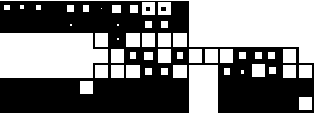
\includegraphics{fig-3.pdf}
  \caption{一个五层网络在学习后的活动状态。底层左侧有 24 个输入单元用于表示<人物1>,右侧有 12 个输入单元用于表示关系。这两组内的白色方块显示了单元的活动状态。第一组中有一个活动单元代表 Colin,第二组中有一个活动单元代表关系“有阿姨”。每组输入单元都完全连接到第二层中各自的 6 个单元组。这些组学习将人物和关系编码为分布式活动模式。第二层完全连接到中间的 12 个单元层,这些单元又连接到倒数第二层的 6 个单元。倒数第二层的活动必须激活正确的输出单元,每个输出单元代表一个特定的<人物2>。在这种情况下,有两个正确答案(用黑点标记),因为 Colin 有两个阿姨。输入单元和输出单元在空间上排列,其中英国人在一行,同构的意大利人紧接在下方。}
  \label{fig-3}
\end{figure}

\begin{figure}
  \centering
  \begingroup
  \tikzset{every picture/.style={scale=0.3}}%
  \begin{tikzpicture}
	\begin{pgfonlayer}{nodelayer}
		\node [style=none] (0) at (-12, 3) {};
		\node [style=none] (1) at (-12, -3) {};
		\node [style=none] (2) at (12, 3) {};
		\node [style=none] (3) at (12, -3) {};
		\node [style=none] (4) at (-11.25, 2.25) {};
		\node [style=none] (5) at (-9.75, 2.25) {};
		\node [style=none] (6) at (-11.25, 0.75) {};
		\node [style=none] (7) at (-9.75, 0.75) {};
		\node [style=none] (8) at (-11.75, -0.25) {};
		\node [style=none] (9) at (-9.5, -0.25) {};
		\node [style=none] (10) at (-11.75, -2.5) {};
		\node [style=none] (11) at (-9.5, -2.5) {};
		\node [style=none] (12) at (-7.25, 2.25) {};
		\node [style=none] (13) at (-5.75, 2.25) {};
		\node [style=none] (14) at (-7.25, 0.75) {};
		\node [style=none] (15) at (-5.75, 0.75) {};
		\node [style=none] (16) at (-7, -1) {};
		\node [style=none] (17) at (-6, -1) {};
		\node [style=none] (18) at (-7, -2) {};
		\node [style=none] (19) at (-6, -2) {};
		\node [style=none] (20) at (1.25, 2) {};
		\node [style=none] (21) at (2.25, 2) {};
		\node [style=none] (22) at (1.25, 1) {};
		\node [style=none] (23) at (2.25, 1) {};
		\node [style=none] (24) at (8.5, 2) {};
		\node [style=none] (25) at (9.5, 2) {};
		\node [style=none] (26) at (8.5, 1) {};
		\node [style=none] (27) at (9.5, 1) {};
		\node [style=none] (28) at (-9.25, 2.25) {};
		\node [style=none] (29) at (-7.75, 2.25) {};
		\node [style=none] (30) at (-9.25, 0.75) {};
		\node [style=none] (31) at (-7.75, 0.75) {};
		\node [style=none] (32) at (-4.75, 1.75) {};
		\node [style=none] (33) at (-4.25, 1.75) {};
		\node [style=none] (34) at (-4.75, 1.25) {};
		\node [style=none] (35) at (-4.25, 1.25) {};
		\node [style=none] (36) at (-9, -1) {};
		\node [style=none] (37) at (-8, -1) {};
		\node [style=none] (38) at (-9, -2) {};
		\node [style=none] (39) at (-8, -2) {};
		\node [style=none] (40) at (-4.75, -1.25) {};
		\node [style=none] (41) at (-4.25, -1.25) {};
		\node [style=none] (42) at (-4.75, -1.75) {};
		\node [style=none] (43) at (-4.25, -1.75) {};
		\node [style=none] (44) at (-3.5, 2.5) {};
		\node [style=none] (45) at (-1.25, 2.5) {};
		\node [style=none] (46) at (-3.5, 0.5) {};
		\node [style=none] (47) at (-1.25, 0.5) {};
		\node [style=none] (48) at (-0.75, 2.25) {};
		\node [style=none] (49) at (0.75, 2.25) {};
		\node [style=none] (50) at (-0.75, 0.75) {};
		\node [style=none] (51) at (0.75, 0.75) {};
		\node [style=none] (52) at (3, 2.25) {};
		\node [style=none] (53) at (4.5, 2.25) {};
		\node [style=none] (54) at (3, 0.75) {};
		\node [style=none] (55) at (4.5, 0.75) {};
		\node [style=none] (56) at (6.25, 2.25) {};
		\node [style=none] (57) at (7.75, 2.25) {};
		\node [style=none] (58) at (6.25, 0.75) {};
		\node [style=none] (59) at (7.75, 0.75) {};
		\node [style=none] (60) at (10.5, 1.75) {};
		\node [style=none] (61) at (11, 1.75) {};
		\node [style=none] (62) at (10.5, 1.25) {};
		\node [style=none] (63) at (11, 1.25) {};
		\node [style=none] (64) at (10.25, -1) {};
		\node [style=none] (65) at (11.25, -1) {};
		\node [style=none] (66) at (10.25, -2) {};
		\node [style=none] (67) at (11.25, -2) {};
		\node [style=none] (68) at (8.5, -1) {};
		\node [style=none] (69) at (9.5, -1) {};
		\node [style=none] (70) at (8.5, -2) {};
		\node [style=none] (71) at (9.5, -2) {};
		\node [style=none] (72) at (-3, -0.75) {};
		\node [style=none] (73) at (-1.5, -0.75) {};
		\node [style=none] (74) at (-3, -2.25) {};
		\node [style=none] (75) at (-1.5, -2.25) {};
		\node [style=none] (76) at (-0.75, -0.75) {};
		\node [style=none] (77) at (0.75, -0.75) {};
		\node [style=none] (78) at (-0.75, -2.25) {};
		\node [style=none] (79) at (0.75, -2.25) {};
		\node [style=none] (80) at (3.25, -1) {};
		\node [style=none] (81) at (4.25, -1) {};
		\node [style=none] (82) at (3.25, -2) {};
		\node [style=none] (83) at (4.25, -2) {};
		\node [style=none] (84) at (6.25, -0.75) {};
		\node [style=none] (85) at (7.75, -0.75) {};
		\node [style=none] (86) at (6.25, -2.25) {};
		\node [style=none] (87) at (7.75, -2.25) {};
		\node [style=none] (88) at (1.25, -1) {};
		\node [style=none] (89) at (2.25, -1) {};
		\node [style=none] (90) at (1.25, -2) {};
		\node [style=none] (91) at (2.25, -2) {};
		\node [style=none] (92) at (5, -1.25) {};
		\node [style=none] (93) at (5.75, -1.25) {};
		\node [style=none] (94) at (5, -1.75) {};
		\node [style=none] (95) at (5.75, -1.75) {};
		\node [style=none] (96) at (5, 1.75) {};
		\node [style=none] (97) at (5.5, 1.75) {};
		\node [style=none] (98) at (5, 1.25) {};
		\node [style=none] (99) at (5.5, 1.25) {};
		\node [style=none] (102) at (-10.5, 6.5) {\rotatebox{90}{Christopher}};
		\node [style=none] (103) at (-8.5, 6.5) {\rotatebox{90}{Andrew}};
		\node [style=none] (104) at (-6.75, 6.5) {\rotatebox{90}{Arthur}};
		\node [style=none] (105) at (-4.75, 6.5) {\rotatebox{90}{James}};
		\node [style=none] (106) at (-2.5, 6.5) {\rotatebox{90}{Charles}};
		\node [style=none] (107) at (0, 6.5) {\rotatebox{90}{Colin}};
		\node [style=none] (108) at (1.5, 6.5) {\rotatebox{90}{Penelope}};
		\node [style=none] (109) at (5.25, 6.5) {\rotatebox{90}{Victoria}};
		\node [style=none] (110) at (7, 6.5) {\rotatebox{90}{Jennifer}};
		\node [style=none] (111) at (9, 6.5) {\rotatebox{90}{Margaret}};
		\node [style=none] (112) at (10.75, 6.5) {\rotatebox{90}{Charlotte}};
		\node [style=none] (113) at (3.75, 6.5) {\rotatebox{90}{Christine}};
		\node [style=none] (114) at (-13, 0) {4};
		\node [style=none] (115) at (-12, -4.25) {};
		\node [style=none] (116) at (-12, -10.25) {};
		\node [style=none] (117) at (12, -4.25) {};
		\node [style=none] (118) at (12, -10.25) {};
		\node [style=none] (119) at (-11.25, -5) {};
		\node [style=none] (120) at (-9.75, -5) {};
		\node [style=none] (121) at (-11.25, -6.5) {};
		\node [style=none] (122) at (-9.75, -6.5) {};
		\node [style=none] (123) at (-11.75, -7.5) {};
		\node [style=none] (124) at (-9.5, -7.5) {};
		\node [style=none] (125) at (-11.75, -9.75) {};
		\node [style=none] (126) at (-9.5, -9.75) {};
		\node [style=none] (127) at (-7.25, -5) {};
		\node [style=none] (128) at (-5.75, -5) {};
		\node [style=none] (129) at (-7.25, -6.5) {};
		\node [style=none] (130) at (-5.75, -6.5) {};
		\node [style=none] (131) at (-7, -8.25) {};
		\node [style=none] (132) at (-6, -8.25) {};
		\node [style=none] (133) at (-7, -9.25) {};
		\node [style=none] (134) at (-6, -9.25) {};
		\node [style=none] (135) at (1.25, -5.25) {};
		\node [style=none] (136) at (2.25, -5.25) {};
		\node [style=none] (137) at (1.25, -6.25) {};
		\node [style=none] (138) at (2.25, -6.25) {};
		\node [style=none] (139) at (8.5, -5.25) {};
		\node [style=none] (140) at (9.5, -5.25) {};
		\node [style=none] (141) at (8.5, -6.25) {};
		\node [style=none] (142) at (9.5, -6.25) {};
		\node [style=none] (143) at (-9.25, -5) {};
		\node [style=none] (144) at (-7.75, -5) {};
		\node [style=none] (145) at (-9.25, -6.5) {};
		\node [style=none] (146) at (-7.75, -6.5) {};
		\node [style=none] (147) at (-4.75, -5.5) {};
		\node [style=none] (148) at (-4.25, -5.5) {};
		\node [style=none] (149) at (-4.75, -6) {};
		\node [style=none] (150) at (-4.25, -6) {};
		\node [style=none] (151) at (-9, -8.25) {};
		\node [style=none] (152) at (-8, -8.25) {};
		\node [style=none] (153) at (-9, -9.25) {};
		\node [style=none] (154) at (-8, -9.25) {};
		\node [style=none] (155) at (-4.75, -8.5) {};
		\node [style=none] (156) at (-4.25, -8.5) {};
		\node [style=none] (157) at (-4.75, -9) {};
		\node [style=none] (158) at (-4.25, -9) {};
		\node [style=none] (159) at (-3.5, -4.75) {};
		\node [style=none] (160) at (-1.25, -4.75) {};
		\node [style=none] (161) at (-3.5, -6.75) {};
		\node [style=none] (162) at (-1.25, -6.75) {};
		\node [style=none] (163) at (-0.75, -5) {};
		\node [style=none] (164) at (0.75, -5) {};
		\node [style=none] (165) at (-0.75, -6.5) {};
		\node [style=none] (166) at (0.75, -6.5) {};
		\node [style=none] (167) at (3, -5) {};
		\node [style=none] (168) at (4.5, -5) {};
		\node [style=none] (169) at (3, -6.5) {};
		\node [style=none] (170) at (4.5, -6.5) {};
		\node [style=none] (171) at (6.25, -5) {};
		\node [style=none] (172) at (7.75, -5) {};
		\node [style=none] (173) at (6.25, -6.5) {};
		\node [style=none] (174) at (7.75, -6.5) {};
		\node [style=none] (175) at (10.5, -5.5) {};
		\node [style=none] (176) at (11, -5.5) {};
		\node [style=none] (177) at (10.5, -6) {};
		\node [style=none] (178) at (11, -6) {};
		\node [style=none] (179) at (10.25, -8.25) {};
		\node [style=none] (180) at (11.25, -8.25) {};
		\node [style=none] (181) at (10.25, -9.25) {};
		\node [style=none] (182) at (11.25, -9.25) {};
		\node [style=none] (183) at (8.5, -8.25) {};
		\node [style=none] (184) at (9.5, -8.25) {};
		\node [style=none] (185) at (8.5, -9.25) {};
		\node [style=none] (186) at (9.5, -9.25) {};
		\node [style=none] (187) at (-3, -8) {};
		\node [style=none] (188) at (-1.5, -8) {};
		\node [style=none] (189) at (-3, -9.5) {};
		\node [style=none] (190) at (-1.5, -9.5) {};
		\node [style=none] (191) at (-0.75, -8) {};
		\node [style=none] (192) at (0.75, -8) {};
		\node [style=none] (193) at (-0.75, -9.5) {};
		\node [style=none] (194) at (0.75, -9.5) {};
		\node [style=none] (195) at (3.25, -8.25) {};
		\node [style=none] (196) at (4.25, -8.25) {};
		\node [style=none] (197) at (3.25, -9.25) {};
		\node [style=none] (198) at (4.25, -9.25) {};
		\node [style=none] (199) at (6.25, -8) {};
		\node [style=none] (200) at (7.75, -8) {};
		\node [style=none] (201) at (6.25, -9.5) {};
		\node [style=none] (202) at (7.75, -9.5) {};
		\node [style=none] (203) at (1.25, -8.25) {};
		\node [style=none] (204) at (2.25, -8.25) {};
		\node [style=none] (205) at (1.25, -9.25) {};
		\node [style=none] (206) at (2.25, -9.25) {};
		\node [style=none] (207) at (5, -8.5) {};
		\node [style=none] (208) at (5.75, -8.5) {};
		\node [style=none] (209) at (5, -9) {};
		\node [style=none] (210) at (5.75, -9) {};
		\node [style=none] (211) at (5, -5.5) {};
		\node [style=none] (212) at (5.5, -5.5) {};
		\node [style=none] (213) at (5, -6) {};
		\node [style=none] (214) at (5.5, -6) {};
		\node [style=none] (215) at (-13, -7.25) {5};
		\node [style=none] (216) at (-12, -11.25) {};
		\node [style=none] (217) at (-12, -17.25) {};
		\node [style=none] (218) at (12, -11.25) {};
		\node [style=none] (219) at (12, -17.25) {};
		\node [style=none] (220) at (-9.25, -12) {};
		\node [style=none] (221) at (-7.75, -12) {};
		\node [style=none] (222) at (-9.25, -13.5) {};
		\node [style=none] (223) at (-7.75, -13.5) {};
		\node [style=none] (224) at (-9, -15) {};
		\node [style=none] (225) at (-7.75, -15) {};
		\node [style=none] (226) at (-9, -16.25) {};
		\node [style=none] (227) at (-7.75, -16.25) {};
		\node [style=none] (228) at (-5.5, -12) {};
		\node [style=none] (229) at (-4, -12) {};
		\node [style=none] (230) at (-5.5, -13.5) {};
		\node [style=none] (231) at (-4, -13.5) {};
		\node [style=none] (232) at (-5.25, -15.25) {};
		\node [style=none] (233) at (-4.25, -15.25) {};
		\node [style=none] (234) at (-5.25, -16.25) {};
		\node [style=none] (235) at (-4.25, -16.25) {};
		\node [style=none] (236) at (1.25, -12.25) {};
		\node [style=none] (237) at (2.25, -12.25) {};
		\node [style=none] (238) at (1.25, -13.25) {};
		\node [style=none] (239) at (2.25, -13.25) {};
		\node [style=none] (240) at (8.5, -12.25) {};
		\node [style=none] (241) at (9.5, -12.25) {};
		\node [style=none] (242) at (8.5, -13.25) {};
		\node [style=none] (243) at (9.5, -13.25) {};
		\node [style=none] (244) at (-11.25, -15) {};
		\node [style=none] (245) at (-9.75, -15) {};
		\node [style=none] (246) at (-11.25, -16.5) {};
		\node [style=none] (247) at (-9.75, -16.5) {};
		\node [style=none] (248) at (-6.75, -12.5) {};
		\node [style=none] (249) at (-6.25, -12.5) {};
		\node [style=none] (250) at (-6.75, -13) {};
		\node [style=none] (251) at (-6.25, -13) {};
		\node [style=none] (256) at (-6.75, -15.5) {};
		\node [style=none] (257) at (-6.25, -15.5) {};
		\node [style=none] (258) at (-6.75, -16) {};
		\node [style=none] (259) at (-6.25, -16) {};
		\node [style=none] (264) at (-0.75, -12) {};
		\node [style=none] (265) at (0.75, -12) {};
		\node [style=none] (266) at (-0.75, -13.5) {};
		\node [style=none] (267) at (0.75, -13.5) {};
		\node [style=none] (268) at (3, -12) {};
		\node [style=none] (269) at (4.5, -12) {};
		\node [style=none] (270) at (3, -13.5) {};
		\node [style=none] (271) at (4.5, -13.5) {};
		\node [style=none] (272) at (6.25, -12) {};
		\node [style=none] (273) at (7.75, -12) {};
		\node [style=none] (274) at (6.25, -13.5) {};
		\node [style=none] (275) at (7.75, -13.5) {};
		\node [style=none] (276) at (10.5, -12.5) {};
		\node [style=none] (277) at (11, -12.5) {};
		\node [style=none] (278) at (10.5, -13) {};
		\node [style=none] (279) at (11, -13) {};
		\node [style=none] (280) at (10.25, -15.25) {};
		\node [style=none] (281) at (11.25, -15.25) {};
		\node [style=none] (282) at (10.25, -16.25) {};
		\node [style=none] (283) at (11.25, -16.25) {};
		\node [style=none] (284) at (8.5, -15.25) {};
		\node [style=none] (285) at (9.5, -15.25) {};
		\node [style=none] (286) at (8.5, -16.25) {};
		\node [style=none] (287) at (9.5, -16.25) {};
		\node [style=none] (292) at (-0.75, -15) {};
		\node [style=none] (293) at (0.75, -15) {};
		\node [style=none] (294) at (-0.75, -16.5) {};
		\node [style=none] (295) at (0.75, -16.5) {};
		\node [style=none] (296) at (3.25, -15.25) {};
		\node [style=none] (297) at (4.25, -15.25) {};
		\node [style=none] (298) at (3.25, -16.25) {};
		\node [style=none] (299) at (4.25, -16.25) {};
		\node [style=none] (300) at (6.25, -15) {};
		\node [style=none] (301) at (7.75, -15) {};
		\node [style=none] (302) at (6.25, -16.5) {};
		\node [style=none] (303) at (7.75, -16.5) {};
		\node [style=none] (304) at (1.25, -15.25) {};
		\node [style=none] (305) at (2.25, -15.25) {};
		\node [style=none] (306) at (1.25, -16.25) {};
		\node [style=none] (307) at (2.25, -16.25) {};
		\node [style=none] (308) at (5, -15.5) {};
		\node [style=none] (309) at (5.75, -15.5) {};
		\node [style=none] (310) at (5, -16) {};
		\node [style=none] (311) at (5.75, -16) {};
		\node [style=none] (312) at (5, -12.5) {};
		\node [style=none] (313) at (5.5, -12.5) {};
		\node [style=none] (314) at (5, -13) {};
		\node [style=none] (315) at (5.5, -13) {};
		\node [style=none] (316) at (-13, -14.25) {6};
		\node [style=none] (317) at (14, 3) {};
		\node [style=none] (318) at (14, -3) {};
		\node [style=none] (319) at (38, 3) {};
		\node [style=none] (320) at (38, -3) {};
		\node [style=none] (321) at (14.75, 2.25) {};
		\node [style=none] (322) at (16.25, 2.25) {};
		\node [style=none] (323) at (14.75, 0.75) {};
		\node [style=none] (324) at (16.25, 0.75) {};
		\node [style=none] (325) at (14.25, -0.25) {};
		\node [style=none] (326) at (16.5, -0.25) {};
		\node [style=none] (327) at (14.25, -2.5) {};
		\node [style=none] (328) at (16.5, -2.5) {};
		\node [style=none] (329) at (18.75, 2.25) {};
		\node [style=none] (330) at (20.25, 2.25) {};
		\node [style=none] (331) at (18.75, 0.75) {};
		\node [style=none] (332) at (20.25, 0.75) {};
		\node [style=none] (333) at (19, -1) {};
		\node [style=none] (334) at (20, -1) {};
		\node [style=none] (335) at (19, -2) {};
		\node [style=none] (336) at (20, -2) {};
		\node [style=none] (337) at (27.25, 2) {};
		\node [style=none] (338) at (28.25, 2) {};
		\node [style=none] (339) at (27.25, 1) {};
		\node [style=none] (340) at (28.25, 1) {};
		\node [style=none] (341) at (34.5, 2) {};
		\node [style=none] (342) at (35.5, 2) {};
		\node [style=none] (343) at (34.5, 1) {};
		\node [style=none] (344) at (35.5, 1) {};
		\node [style=none] (345) at (16.75, 2.25) {};
		\node [style=none] (346) at (18.25, 2.25) {};
		\node [style=none] (347) at (16.75, 0.75) {};
		\node [style=none] (348) at (18.25, 0.75) {};
		\node [style=none] (349) at (21.25, 1.75) {};
		\node [style=none] (350) at (21.75, 1.75) {};
		\node [style=none] (351) at (21.25, 1.25) {};
		\node [style=none] (352) at (21.75, 1.25) {};
		\node [style=none] (353) at (17, -1) {};
		\node [style=none] (354) at (18, -1) {};
		\node [style=none] (355) at (17, -2) {};
		\node [style=none] (356) at (18, -2) {};
		\node [style=none] (357) at (21.25, -1.25) {};
		\node [style=none] (358) at (21.75, -1.25) {};
		\node [style=none] (359) at (21.25, -1.75) {};
		\node [style=none] (360) at (21.75, -1.75) {};
		\node [style=none] (361) at (22.5, 2.5) {};
		\node [style=none] (362) at (24.75, 2.5) {};
		\node [style=none] (363) at (22.5, 0.5) {};
		\node [style=none] (364) at (24.75, 0.5) {};
		\node [style=none] (365) at (25.25, 2.25) {};
		\node [style=none] (366) at (26.75, 2.25) {};
		\node [style=none] (367) at (25.25, 0.75) {};
		\node [style=none] (368) at (26.75, 0.75) {};
		\node [style=none] (369) at (29, 2.25) {};
		\node [style=none] (370) at (30.5, 2.25) {};
		\node [style=none] (371) at (29, 0.75) {};
		\node [style=none] (372) at (30.5, 0.75) {};
		\node [style=none] (373) at (32.25, 2.25) {};
		\node [style=none] (374) at (33.75, 2.25) {};
		\node [style=none] (375) at (32.25, 0.75) {};
		\node [style=none] (376) at (33.75, 0.75) {};
		\node [style=none] (377) at (36.5, 1.75) {};
		\node [style=none] (378) at (37, 1.75) {};
		\node [style=none] (379) at (36.5, 1.25) {};
		\node [style=none] (380) at (37, 1.25) {};
		\node [style=none] (381) at (36.25, -1) {};
		\node [style=none] (382) at (37.25, -1) {};
		\node [style=none] (383) at (36.25, -2) {};
		\node [style=none] (384) at (37.25, -2) {};
		\node [style=none] (385) at (34.5, -1) {};
		\node [style=none] (386) at (35.5, -1) {};
		\node [style=none] (387) at (34.5, -2) {};
		\node [style=none] (388) at (35.5, -2) {};
		\node [style=none] (389) at (23, -0.75) {};
		\node [style=none] (390) at (24.5, -0.75) {};
		\node [style=none] (391) at (23, -2.25) {};
		\node [style=none] (392) at (24.5, -2.25) {};
		\node [style=none] (393) at (25.25, -0.75) {};
		\node [style=none] (394) at (26.75, -0.75) {};
		\node [style=none] (395) at (25.25, -2.25) {};
		\node [style=none] (396) at (26.75, -2.25) {};
		\node [style=none] (397) at (29.25, -1) {};
		\node [style=none] (398) at (30.25, -1) {};
		\node [style=none] (399) at (29.25, -2) {};
		\node [style=none] (400) at (30.25, -2) {};
		\node [style=none] (401) at (32.25, -0.75) {};
		\node [style=none] (402) at (33.75, -0.75) {};
		\node [style=none] (403) at (32.25, -2.25) {};
		\node [style=none] (404) at (33.75, -2.25) {};
		\node [style=none] (405) at (27.25, -1) {};
		\node [style=none] (406) at (28.25, -1) {};
		\node [style=none] (407) at (27.25, -2) {};
		\node [style=none] (408) at (28.25, -2) {};
		\node [style=none] (409) at (31, -1.25) {};
		\node [style=none] (410) at (31.75, -1.25) {};
		\node [style=none] (411) at (31, -1.75) {};
		\node [style=none] (412) at (31.75, -1.75) {};
		\node [style=none] (413) at (31, 1.75) {};
		\node [style=none] (414) at (31.5, 1.75) {};
		\node [style=none] (415) at (31, 1.25) {};
		\node [style=none] (416) at (31.5, 1.25) {};
		\node [style=none] (417) at (15.5, 6.5) {\rotatebox{90}{Christopher}};
		\node [style=none] (418) at (17.5, 6.5) {\rotatebox{90}{Andrew}};
		\node [style=none] (419) at (19.25, 6.5) {\rotatebox{90}{Arthur}};
		\node [style=none] (420) at (21.25, 6.5) {\rotatebox{90}{James}};
		\node [style=none] (421) at (23.5, 6.5) {\rotatebox{90}{Charles}};
		\node [style=none] (422) at (26, 6.5) {\rotatebox{90}{Colin}};
		\node [style=none] (423) at (27.5, 6.5) {\rotatebox{90}{Penelope}};
		\node [style=none] (424) at (31.25, 6.5) {\rotatebox{90}{Victoria}};
		\node [style=none] (425) at (33, 6.5) {\rotatebox{90}{Jennifer}};
		\node [style=none] (426) at (35, 6.5) {\rotatebox{90}{Margaret}};
		\node [style=none] (427) at (36.75, 6.5) {\rotatebox{90}{Charlotte}};
		\node [style=none] (428) at (29.75, 6.5) {\rotatebox{90}{Christine}};
		\node [style=none] (429) at (39, 0) {1};
		\node [style=none] (430) at (14, -4.25) {};
		\node [style=none] (431) at (14, -10.25) {};
		\node [style=none] (432) at (38, -4.25) {};
		\node [style=none] (433) at (38, -10.25) {};
		\node [style=none] (434) at (14.75, -5) {};
		\node [style=none] (435) at (16.25, -5) {};
		\node [style=none] (436) at (14.75, -6.5) {};
		\node [style=none] (437) at (16.25, -6.5) {};
		\node [style=none] (438) at (14.25, -7.5) {};
		\node [style=none] (439) at (16.5, -7.5) {};
		\node [style=none] (440) at (14.25, -9.75) {};
		\node [style=none] (441) at (16.5, -9.75) {};
		\node [style=none] (442) at (18.75, -5) {};
		\node [style=none] (443) at (20.25, -5) {};
		\node [style=none] (444) at (18.75, -6.5) {};
		\node [style=none] (445) at (20.25, -6.5) {};
		\node [style=none] (446) at (19, -8.25) {};
		\node [style=none] (447) at (20, -8.25) {};
		\node [style=none] (448) at (19, -9.25) {};
		\node [style=none] (449) at (20, -9.25) {};
		\node [style=none] (450) at (27.25, -5.25) {};
		\node [style=none] (451) at (28.25, -5.25) {};
		\node [style=none] (452) at (27.25, -6.25) {};
		\node [style=none] (453) at (28.25, -6.25) {};
		\node [style=none] (454) at (34.5, -5.25) {};
		\node [style=none] (455) at (35.5, -5.25) {};
		\node [style=none] (456) at (34.5, -6.25) {};
		\node [style=none] (457) at (35.5, -6.25) {};
		\node [style=none] (458) at (16.75, -5) {};
		\node [style=none] (459) at (18.25, -5) {};
		\node [style=none] (460) at (16.75, -6.5) {};
		\node [style=none] (461) at (18.25, -6.5) {};
		\node [style=none] (462) at (21.25, -5.5) {};
		\node [style=none] (463) at (21.75, -5.5) {};
		\node [style=none] (464) at (21.25, -6) {};
		\node [style=none] (465) at (21.75, -6) {};
		\node [style=none] (466) at (17, -8.25) {};
		\node [style=none] (467) at (18, -8.25) {};
		\node [style=none] (468) at (17, -9.25) {};
		\node [style=none] (469) at (18, -9.25) {};
		\node [style=none] (470) at (21.25, -8.5) {};
		\node [style=none] (471) at (21.75, -8.5) {};
		\node [style=none] (472) at (21.25, -9) {};
		\node [style=none] (473) at (21.75, -9) {};
		\node [style=none] (474) at (22.5, -4.75) {};
		\node [style=none] (475) at (24.75, -4.75) {};
		\node [style=none] (476) at (22.5, -6.75) {};
		\node [style=none] (477) at (24.75, -6.75) {};
		\node [style=none] (478) at (25.25, -5) {};
		\node [style=none] (479) at (26.75, -5) {};
		\node [style=none] (480) at (25.25, -6.5) {};
		\node [style=none] (481) at (26.75, -6.5) {};
		\node [style=none] (482) at (29, -5) {};
		\node [style=none] (483) at (30.5, -5) {};
		\node [style=none] (484) at (29, -6.5) {};
		\node [style=none] (485) at (30.5, -6.5) {};
		\node [style=none] (486) at (32.25, -5) {};
		\node [style=none] (487) at (33.75, -5) {};
		\node [style=none] (488) at (32.25, -6.5) {};
		\node [style=none] (489) at (33.75, -6.5) {};
		\node [style=none] (490) at (36.5, -5.5) {};
		\node [style=none] (491) at (37, -5.5) {};
		\node [style=none] (492) at (36.5, -6) {};
		\node [style=none] (493) at (37, -6) {};
		\node [style=none] (494) at (36.25, -8.25) {};
		\node [style=none] (495) at (37.25, -8.25) {};
		\node [style=none] (496) at (36.25, -9.25) {};
		\node [style=none] (497) at (37.25, -9.25) {};
		\node [style=none] (498) at (34.5, -8.25) {};
		\node [style=none] (499) at (35.5, -8.25) {};
		\node [style=none] (500) at (34.5, -9.25) {};
		\node [style=none] (501) at (35.5, -9.25) {};
		\node [style=none] (502) at (23, -8) {};
		\node [style=none] (503) at (24.5, -8) {};
		\node [style=none] (504) at (23, -9.5) {};
		\node [style=none] (505) at (24.5, -9.5) {};
		\node [style=none] (506) at (25.25, -8) {};
		\node [style=none] (507) at (26.75, -8) {};
		\node [style=none] (508) at (25.25, -9.5) {};
		\node [style=none] (509) at (26.75, -9.5) {};
		\node [style=none] (510) at (29.25, -8.25) {};
		\node [style=none] (511) at (30.25, -8.25) {};
		\node [style=none] (512) at (29.25, -9.25) {};
		\node [style=none] (513) at (30.25, -9.25) {};
		\node [style=none] (514) at (32.25, -8) {};
		\node [style=none] (515) at (33.75, -8) {};
		\node [style=none] (516) at (32.25, -9.5) {};
		\node [style=none] (517) at (33.75, -9.5) {};
		\node [style=none] (518) at (27.25, -8.25) {};
		\node [style=none] (519) at (28.25, -8.25) {};
		\node [style=none] (520) at (27.25, -9.25) {};
		\node [style=none] (521) at (28.25, -9.25) {};
		\node [style=none] (522) at (31, -8.5) {};
		\node [style=none] (523) at (31.75, -8.5) {};
		\node [style=none] (524) at (31, -9) {};
		\node [style=none] (525) at (31.75, -9) {};
		\node [style=none] (526) at (31, -5.5) {};
		\node [style=none] (527) at (31.5, -5.5) {};
		\node [style=none] (528) at (31, -6) {};
		\node [style=none] (529) at (31.5, -6) {};
		\node [style=none] (530) at (39, -7.25) {2};
		\node [style=none] (531) at (14, -11.25) {};
		\node [style=none] (532) at (14, -17.25) {};
		\node [style=none] (533) at (38, -11.25) {};
		\node [style=none] (534) at (38, -17.25) {};
		\node [style=none] (535) at (14.75, -12) {};
		\node [style=none] (536) at (16.25, -12) {};
		\node [style=none] (537) at (14.75, -13.5) {};
		\node [style=none] (538) at (16.25, -13.5) {};
		\node [style=none] (539) at (14.25, -14.5) {};
		\node [style=none] (540) at (16.5, -14.5) {};
		\node [style=none] (541) at (14.25, -16.75) {};
		\node [style=none] (542) at (16.5, -16.75) {};
		\node [style=none] (543) at (18.75, -12) {};
		\node [style=none] (544) at (20.25, -12) {};
		\node [style=none] (545) at (18.75, -13.5) {};
		\node [style=none] (546) at (20.25, -13.5) {};
		\node [style=none] (547) at (19, -15.25) {};
		\node [style=none] (548) at (20, -15.25) {};
		\node [style=none] (549) at (19, -16.25) {};
		\node [style=none] (550) at (20, -16.25) {};
		\node [style=none] (551) at (27.25, -12.25) {};
		\node [style=none] (552) at (28.25, -12.25) {};
		\node [style=none] (553) at (27.25, -13.25) {};
		\node [style=none] (554) at (28.25, -13.25) {};
		\node [style=none] (555) at (34.5, -12.25) {};
		\node [style=none] (556) at (35.5, -12.25) {};
		\node [style=none] (557) at (34.5, -13.25) {};
		\node [style=none] (558) at (35.5, -13.25) {};
		\node [style=none] (559) at (16.75, -12) {};
		\node [style=none] (560) at (18.25, -12) {};
		\node [style=none] (561) at (16.75, -13.5) {};
		\node [style=none] (562) at (18.25, -13.5) {};
		\node [style=none] (563) at (21.25, -12.5) {};
		\node [style=none] (564) at (21.75, -12.5) {};
		\node [style=none] (565) at (21.25, -13) {};
		\node [style=none] (566) at (21.75, -13) {};
		\node [style=none] (567) at (17, -15.25) {};
		\node [style=none] (568) at (18, -15.25) {};
		\node [style=none] (569) at (17, -16.25) {};
		\node [style=none] (570) at (18, -16.25) {};
		\node [style=none] (571) at (21.25, -15.5) {};
		\node [style=none] (572) at (21.75, -15.5) {};
		\node [style=none] (573) at (21.25, -16) {};
		\node [style=none] (574) at (21.75, -16) {};
		\node [style=none] (575) at (22.5, -11.75) {};
		\node [style=none] (576) at (24.75, -11.75) {};
		\node [style=none] (577) at (22.5, -13.75) {};
		\node [style=none] (578) at (24.75, -13.75) {};
		\node [style=none] (579) at (25.25, -12) {};
		\node [style=none] (580) at (26.75, -12) {};
		\node [style=none] (581) at (25.25, -13.5) {};
		\node [style=none] (582) at (26.75, -13.5) {};
		\node [style=none] (583) at (29, -12) {};
		\node [style=none] (584) at (30.5, -12) {};
		\node [style=none] (585) at (29, -13.5) {};
		\node [style=none] (586) at (30.5, -13.5) {};
		\node [style=none] (587) at (32.25, -12) {};
		\node [style=none] (588) at (33.75, -12) {};
		\node [style=none] (589) at (32.25, -13.5) {};
		\node [style=none] (590) at (33.75, -13.5) {};
		\node [style=none] (591) at (36.5, -12.5) {};
		\node [style=none] (592) at (37, -12.5) {};
		\node [style=none] (593) at (36.5, -13) {};
		\node [style=none] (594) at (37, -13) {};
		\node [style=none] (595) at (36.25, -15.25) {};
		\node [style=none] (596) at (37.25, -15.25) {};
		\node [style=none] (597) at (36.25, -16.25) {};
		\node [style=none] (598) at (37.25, -16.25) {};
		\node [style=none] (599) at (34.5, -15.25) {};
		\node [style=none] (600) at (35.5, -15.25) {};
		\node [style=none] (601) at (34.5, -16.25) {};
		\node [style=none] (602) at (35.5, -16.25) {};
		\node [style=none] (603) at (23, -15) {};
		\node [style=none] (604) at (24.5, -15) {};
		\node [style=none] (605) at (23, -16.5) {};
		\node [style=none] (606) at (24.5, -16.5) {};
		\node [style=none] (607) at (25.25, -15) {};
		\node [style=none] (608) at (26.75, -15) {};
		\node [style=none] (609) at (25.25, -16.5) {};
		\node [style=none] (610) at (26.75, -16.5) {};
		\node [style=none] (611) at (29.25, -15.25) {};
		\node [style=none] (612) at (30.25, -15.25) {};
		\node [style=none] (613) at (29.25, -16.25) {};
		\node [style=none] (614) at (30.25, -16.25) {};
		\node [style=none] (615) at (32.25, -15) {};
		\node [style=none] (616) at (33.75, -15) {};
		\node [style=none] (617) at (32.25, -16.5) {};
		\node [style=none] (618) at (33.75, -16.5) {};
		\node [style=none] (619) at (27.25, -15.25) {};
		\node [style=none] (620) at (28.25, -15.25) {};
		\node [style=none] (621) at (27.25, -16.25) {};
		\node [style=none] (622) at (28.25, -16.25) {};
		\node [style=none] (623) at (31, -15.5) {};
		\node [style=none] (624) at (31.75, -15.5) {};
		\node [style=none] (625) at (31, -16) {};
		\node [style=none] (626) at (31.75, -16) {};
		\node [style=none] (627) at (31, -12.5) {};
		\node [style=none] (628) at (31.5, -12.5) {};
		\node [style=none] (629) at (31, -13) {};
		\node [style=none] (630) at (31.5, -13) {};
		\node [style=none] (631) at (39, -14.25) {3};
		\node [style=none] (632) at (-11.25, -12) {};
		\node [style=none] (633) at (-9.75, -12) {};
		\node [style=none] (634) at (-11.25, -13.5) {};
		\node [style=none] (635) at (-9.75, -13.5) {};
	\end{pgfonlayer}
	\begin{pgfonlayer}{edgelayer}
		\draw [style=gray box] (2.center)
			 to (3.center)
			 to (1.center)
			 to (0.center)
			 to cycle;
		\draw [style=black box] (6.center)
			 to (4.center)
			 to (5.center)
			 to (7.center)
			 to cycle;
		\draw [style=black box] (10.center)
			 to (8.center)
			 to (9.center)
			 to (11.center)
			 to cycle;
		\draw [style=black box] (14.center)
			 to (12.center)
			 to (13.center)
			 to (15.center)
			 to cycle;
		\draw [style=black box] (18.center)
			 to (16.center)
			 to (17.center)
			 to (19.center)
			 to cycle;
		\draw [style=black box] (22.center)
			 to (20.center)
			 to (21.center)
			 to (23.center)
			 to cycle;
		\draw [style=black box] (26.center)
			 to (24.center)
			 to (25.center)
			 to (27.center)
			 to cycle;
		\draw [style=white box] (30.center)
			 to (28.center)
			 to (29.center)
			 to (31.center)
			 to cycle;
		\draw [style=white box] (34.center)
			 to (32.center)
			 to (33.center)
			 to (35.center)
			 to cycle;
		\draw [style=white box] (38.center)
			 to (36.center)
			 to (37.center)
			 to (39.center)
			 to cycle;
		\draw [style=white box] (42.center)
			 to (40.center)
			 to (41.center)
			 to (43.center)
			 to cycle;
		\draw [style=white box] (46.center)
			 to (44.center)
			 to (45.center)
			 to (47.center)
			 to cycle;
		\draw [style=white box] (50.center)
			 to (48.center)
			 to (49.center)
			 to (51.center)
			 to cycle;
		\draw [style=white box] (54.center)
			 to (52.center)
			 to (53.center)
			 to (55.center)
			 to cycle;
		\draw [style=white box] (58.center)
			 to (56.center)
			 to (57.center)
			 to (59.center)
			 to cycle;
		\draw [style=white box] (62.center)
			 to (60.center)
			 to (61.center)
			 to (63.center)
			 to cycle;
		\draw [style=black box] (66.center)
			 to (64.center)
			 to (65.center)
			 to (67.center)
			 to cycle;
		\draw [style=black box] (70.center)
			 to (68.center)
			 to (69.center)
			 to (71.center)
			 to cycle;
		\draw [style=white box] (74.center)
			 to (72.center)
			 to (73.center)
			 to (75.center)
			 to cycle;
		\draw [style=white box] (78.center)
			 to (76.center)
			 to (77.center)
			 to (79.center)
			 to cycle;
		\draw [style=white box] (82.center)
			 to (80.center)
			 to (81.center)
			 to (83.center)
			 to cycle;
		\draw [style=white box] (86.center)
			 to (84.center)
			 to (85.center)
			 to (87.center)
			 to cycle;
		\draw [style=black box] (91.center)
			 to (90.center)
			 to (88.center)
			 to (89.center)
			 to cycle;
		\draw [style=black box] (92.center)
			 to (93.center)
			 to (95.center)
			 to (94.center)
			 to cycle;
		\draw [style=white box] (96.center)
			 to (97.center)
			 to (99.center)
			 to (98.center)
			 to cycle;
		\draw [style=gray box] (117.center)
			 to (118.center)
			 to (116.center)
			 to (115.center)
			 to cycle;
		\draw [style=black box] (121.center)
			 to (119.center)
			 to (120.center)
			 to (122.center)
			 to cycle;
		\draw [style=black box] (125.center) to (123.center);
		\draw [style=black box] (123.center) to (124.center);
		\draw [style=black box] (124.center) to (126.center);
		\draw [style=black box] (126.center) to (125.center);
		\draw [style=black box] (129.center) to (127.center);
		\draw [style=black box] (127.center) to (128.center);
		\draw [style=black box] (128.center) to (130.center);
		\draw [style=black box] (130.center) to (129.center);
		\draw [style=black box] (133.center) to (131.center);
		\draw [style=black box] (131.center) to (132.center);
		\draw [style=black box] (132.center) to (134.center);
		\draw [style=black box] (134.center) to (133.center);
		\draw [style=black box] (137.center) to (135.center);
		\draw [style=black box] (135.center) to (136.center);
		\draw [style=black box] (136.center) to (138.center);
		\draw [style=black box] (138.center) to (137.center);
		\draw [style=black box] (141.center)
			 to (139.center)
			 to (140.center)
			 to (142.center)
			 to cycle;
		\draw [style=white box] (145.center)
			 to (143.center)
			 to (144.center)
			 to (146.center)
			 to cycle;
		\draw [style=white box] (147.center)
			 to (148.center)
			 to (150.center)
			 to (149.center)
			 to cycle;
		\draw [style=white box] (153.center) to (151.center);
		\draw [style=white box] (151.center) to (152.center);
		\draw [style=white box] (152.center) to (154.center);
		\draw [style=white box] (154.center) to (153.center);
		\draw [style=white box] (157.center) to (155.center);
		\draw [style=white box] (155.center) to (156.center);
		\draw [style=white box] (156.center) to (158.center);
		\draw [style=white box] (158.center) to (157.center);
		\draw [style=white box] (161.center) to (159.center);
		\draw [style=white box] (159.center) to (160.center);
		\draw [style=white box] (160.center) to (162.center);
		\draw [style=white box] (162.center) to (161.center);
		\draw [style=white box] (165.center) to (163.center);
		\draw [style=white box] (163.center) to (164.center);
		\draw [style=white box] (164.center) to (166.center);
		\draw [style=white box] (166.center) to (165.center);
		\draw [style=white box] (169.center) to (167.center);
		\draw [style=white box] (167.center) to (168.center);
		\draw [style=white box] (168.center) to (170.center);
		\draw [style=white box] (170.center) to (169.center);
		\draw [style=white box] (173.center) to (171.center);
		\draw [style=white box] (171.center) to (172.center);
		\draw [style=white box] (172.center) to (174.center);
		\draw [style=white box] (174.center) to (173.center);
		\draw [style=white box] (177.center) to (175.center);
		\draw [style=white box] (175.center) to (176.center);
		\draw [style=white box] (176.center) to (178.center);
		\draw [style=white box] (178.center) to (177.center);
		\draw [style=black box] (181.center) to (179.center);
		\draw [style=black box] (179.center) to (180.center);
		\draw [style=black box] (180.center) to (182.center);
		\draw [style=black box] (182.center) to (181.center);
		\draw [style=black box] (185.center) to (183.center);
		\draw [style=black box] (183.center) to (184.center);
		\draw [style=black box] (184.center) to (186.center);
		\draw [style=black box] (186.center) to (185.center);
		\draw [style=white box] (189.center) to (187.center);
		\draw [style=white box] (187.center) to (188.center);
		\draw [style=white box] (188.center) to (190.center);
		\draw [style=white box] (190.center) to (189.center);
		\draw [style=white box] (193.center) to (191.center);
		\draw [style=white box] (191.center) to (192.center);
		\draw [style=white box] (192.center) to (194.center);
		\draw [style=white box] (194.center) to (193.center);
		\draw [style=white box] (197.center) to (195.center);
		\draw [style=white box] (195.center) to (196.center);
		\draw [style=white box] (196.center) to (198.center);
		\draw [style=white box] (198.center) to (197.center);
		\draw [style=white box] (201.center) to (199.center);
		\draw [style=white box] (199.center) to (200.center);
		\draw [style=white box] (200.center) to (202.center);
		\draw [style=white box] (202.center) to (201.center);
		\draw [style=black box] (206.center)
			 to (205.center)
			 to (203.center)
			 to (204.center)
			 to cycle;
		\draw [style=black box] (207.center)
			 to (208.center)
			 to (210.center)
			 to (209.center)
			 to cycle;
		\draw [style=white box] (211.center)
			 to (212.center)
			 to (214.center)
			 to (213.center)
			 to cycle;
		\draw [style=gray box] (218.center)
			 to (219.center)
			 to (217.center)
			 to (216.center)
			 to cycle;
		\draw [style=black box] (222.center)
			 to (220.center)
			 to (221.center)
			 to (223.center)
			 to cycle;
		\draw [style=black box] (224.center)
			 to (225.center)
			 to (227.center)
			 to (226.center)
			 to cycle;
		\draw [style=black box] (229.center)
			 to (231.center)
			 to (230.center)
			 to (228.center)
			 to cycle;
		\draw [style=black box] (232.center)
			 to (233.center)
			 to (235.center)
			 to (234.center)
			 to cycle;
		\draw [style=black box] (238.center) to (236.center);
		\draw [style=black box] (236.center) to (237.center);
		\draw [style=black box] (237.center) to (239.center);
		\draw [style=black box] (239.center) to (238.center);
		\draw [style=black box] (242.center)
			 to (240.center)
			 to (241.center)
			 to (243.center)
			 to cycle;
		\draw [style=white box] (246.center)
			 to (244.center)
			 to (245.center)
			 to (247.center)
			 to cycle;
		\draw [style=white box] (250.center)
			 to (248.center)
			 to (249.center)
			 to (251.center)
			 to cycle;
		\draw [style=white box] (258.center)
			 to (256.center)
			 to (257.center)
			 to (259.center)
			 to cycle;
		\draw [style=white box] (266.center) to (264.center);
		\draw [style=white box] (264.center) to (265.center);
		\draw [style=white box] (265.center) to (267.center);
		\draw [style=white box] (267.center) to (266.center);
		\draw [style=white box] (270.center) to (268.center);
		\draw [style=white box] (268.center) to (269.center);
		\draw [style=white box] (269.center) to (271.center);
		\draw [style=white box] (271.center) to (270.center);
		\draw [style=white box] (274.center) to (272.center);
		\draw [style=white box] (272.center) to (273.center);
		\draw [style=white box] (273.center) to (275.center);
		\draw [style=white box] (275.center) to (274.center);
		\draw [style=white box] (278.center) to (276.center);
		\draw [style=white box] (276.center) to (277.center);
		\draw [style=white box] (277.center) to (279.center);
		\draw [style=white box] (279.center) to (278.center);
		\draw [style=black box] (282.center) to (280.center);
		\draw [style=black box] (280.center) to (281.center);
		\draw [style=black box] (281.center) to (283.center);
		\draw [style=black box] (283.center) to (282.center);
		\draw [style=black box] (286.center) to (284.center);
		\draw [style=black box] (284.center) to (285.center);
		\draw [style=black box] (285.center) to (287.center);
		\draw [style=black box] (287.center) to (286.center);
		\draw [style=white box] (294.center) to (292.center);
		\draw [style=white box] (292.center) to (293.center);
		\draw [style=white box] (293.center) to (295.center);
		\draw [style=white box] (295.center) to (294.center);
		\draw [style=white box] (298.center) to (296.center);
		\draw [style=white box] (296.center) to (297.center);
		\draw [style=white box] (297.center) to (299.center);
		\draw [style=white box] (299.center) to (298.center);
		\draw [style=white box] (302.center) to (300.center);
		\draw [style=white box] (300.center) to (301.center);
		\draw [style=white box] (301.center) to (303.center);
		\draw [style=white box] (303.center) to (302.center);
		\draw [style=black box] (307.center)
			 to (306.center)
			 to (304.center)
			 to (305.center)
			 to cycle;
		\draw [style=black box] (308.center)
			 to (309.center)
			 to (311.center)
			 to (310.center)
			 to cycle;
		\draw [style=white box] (312.center)
			 to (313.center)
			 to (315.center)
			 to (314.center)
			 to cycle;
		\draw [style=gray box] (319.center)
			 to (320.center)
			 to (318.center)
			 to (317.center)
			 to cycle;
		\draw [style=black box] (323.center)
			 to (321.center)
			 to (322.center)
			 to (324.center)
			 to cycle;
		\draw [style=black box] (327.center) to (325.center);
		\draw [style=black box] (325.center) to (326.center);
		\draw [style=black box] (326.center) to (328.center);
		\draw [style=black box] (328.center) to (327.center);
		\draw [style=black box] (331.center) to (329.center);
		\draw [style=black box] (329.center) to (330.center);
		\draw [style=black box] (330.center) to (332.center);
		\draw [style=black box] (332.center) to (331.center);
		\draw [style=black box] (335.center) to (333.center);
		\draw [style=black box] (333.center) to (334.center);
		\draw [style=black box] (334.center) to (336.center);
		\draw [style=black box] (336.center) to (335.center);
		\draw [style=black box] (339.center) to (337.center);
		\draw [style=black box] (337.center) to (338.center);
		\draw [style=black box] (338.center) to (340.center);
		\draw [style=black box] (340.center) to (339.center);
		\draw [style=black box] (343.center)
			 to (341.center)
			 to (342.center)
			 to (344.center)
			 to cycle;
		\draw [style=white box] (347.center)
			 to (345.center)
			 to (346.center)
			 to (348.center)
			 to cycle;
		\draw [style=white box] (351.center) to (349.center);
		\draw [style=white box] (349.center) to (350.center);
		\draw [style=white box] (350.center) to (352.center);
		\draw [style=white box] (352.center) to (351.center);
		\draw [style=white box] (355.center) to (353.center);
		\draw [style=white box] (353.center) to (354.center);
		\draw [style=white box] (354.center) to (356.center);
		\draw [style=white box] (356.center) to (355.center);
		\draw [style=white box] (359.center) to (357.center);
		\draw [style=white box] (357.center) to (358.center);
		\draw [style=white box] (358.center) to (360.center);
		\draw [style=white box] (360.center) to (359.center);
		\draw [style=white box] (363.center) to (361.center);
		\draw [style=white box] (361.center) to (362.center);
		\draw [style=white box] (362.center) to (364.center);
		\draw [style=white box] (364.center) to (363.center);
		\draw [style=white box] (367.center) to (365.center);
		\draw [style=white box] (365.center) to (366.center);
		\draw [style=white box] (366.center) to (368.center);
		\draw [style=white box] (368.center) to (367.center);
		\draw [style=white box] (371.center) to (369.center);
		\draw [style=white box] (369.center) to (370.center);
		\draw [style=white box] (370.center) to (372.center);
		\draw [style=white box] (372.center) to (371.center);
		\draw [style=white box] (375.center) to (373.center);
		\draw [style=white box] (373.center) to (374.center);
		\draw [style=white box] (374.center) to (376.center);
		\draw [style=white box] (376.center) to (375.center);
		\draw [style=white box] (379.center) to (377.center);
		\draw [style=white box] (377.center) to (378.center);
		\draw [style=white box] (378.center) to (380.center);
		\draw [style=white box] (380.center) to (379.center);
		\draw [style=black box] (383.center) to (381.center);
		\draw [style=black box] (381.center) to (382.center);
		\draw [style=black box] (382.center) to (384.center);
		\draw [style=black box] (384.center) to (383.center);
		\draw [style=black box] (387.center) to (385.center);
		\draw [style=black box] (385.center) to (386.center);
		\draw [style=black box] (386.center) to (388.center);
		\draw [style=black box] (388.center) to (387.center);
		\draw [style=white box] (391.center) to (389.center);
		\draw [style=white box] (389.center) to (390.center);
		\draw [style=white box] (390.center) to (392.center);
		\draw [style=white box] (392.center) to (391.center);
		\draw [style=white box] (395.center) to (393.center);
		\draw [style=white box] (393.center) to (394.center);
		\draw [style=white box] (394.center) to (396.center);
		\draw [style=white box] (396.center) to (395.center);
		\draw [style=white box] (399.center) to (397.center);
		\draw [style=white box] (397.center) to (398.center);
		\draw [style=white box] (398.center) to (400.center);
		\draw [style=white box] (400.center) to (399.center);
		\draw [style=white box] (403.center) to (401.center);
		\draw [style=white box] (401.center) to (402.center);
		\draw [style=white box] (402.center) to (404.center);
		\draw [style=white box] (404.center) to (403.center);
		\draw [style=black box] (408.center)
			 to (407.center)
			 to (405.center)
			 to (406.center)
			 to cycle;
		\draw [style=black box] (409.center)
			 to (410.center)
			 to (412.center)
			 to (411.center)
			 to cycle;
		\draw [style=white box] (413.center)
			 to (414.center)
			 to (416.center)
			 to (415.center)
			 to cycle;
		\draw [style=gray box] (431.center)
			 to (430.center)
			 to (432.center)
			 to (433.center)
			 to cycle;
		\draw [style=black box] (436.center) to (434.center);
		\draw [style=black box] (434.center) to (435.center);
		\draw [style=black box] (435.center) to (437.center);
		\draw [style=black box] (437.center) to (436.center);
		\draw [style=black box] (440.center) to (438.center);
		\draw [style=black box] (438.center) to (439.center);
		\draw [style=black box] (439.center) to (441.center);
		\draw [style=black box] (441.center) to (440.center);
		\draw [style=black box] (444.center) to (442.center);
		\draw [style=black box] (442.center) to (443.center);
		\draw [style=black box] (443.center) to (445.center);
		\draw [style=black box] (445.center) to (444.center);
		\draw [style=black box] (448.center) to (446.center);
		\draw [style=black box] (446.center) to (447.center);
		\draw [style=black box] (447.center) to (449.center);
		\draw [style=black box] (449.center) to (448.center);
		\draw [style=black box] (452.center) to (450.center);
		\draw [style=black box] (450.center) to (451.center);
		\draw [style=black box] (451.center) to (453.center);
		\draw [style=black box] (453.center) to (452.center);
		\draw [style=black box] (456.center) to (454.center);
		\draw [style=black box] (454.center) to (455.center);
		\draw [style=black box] (455.center) to (457.center);
		\draw [style=black box] (457.center) to (456.center);
		\draw [style=white box] (460.center) to (458.center);
		\draw [style=white box] (458.center) to (459.center);
		\draw [style=white box] (459.center) to (461.center);
		\draw [style=white box] (461.center) to (460.center);
		\draw [style=white box] (462.center)
			 to (463.center)
			 to (465.center)
			 to (464.center)
			 to cycle;
		\draw [style=white box] (468.center) to (466.center);
		\draw [style=white box] (466.center) to (467.center);
		\draw [style=white box] (467.center) to (469.center);
		\draw [style=white box] (469.center) to (468.center);
		\draw [style=white box] (472.center) to (470.center);
		\draw [style=white box] (470.center) to (471.center);
		\draw [style=white box] (471.center) to (473.center);
		\draw [style=white box] (473.center) to (472.center);
		\draw [style=white box] (476.center) to (474.center);
		\draw [style=white box] (474.center) to (475.center);
		\draw [style=white box] (475.center) to (477.center);
		\draw [style=white box] (477.center) to (476.center);
		\draw [style=white box] (480.center) to (478.center);
		\draw [style=white box] (478.center) to (479.center);
		\draw [style=white box] (479.center) to (481.center);
		\draw [style=white box] (481.center) to (480.center);
		\draw [style=white box] (484.center) to (482.center);
		\draw [style=white box] (482.center) to (483.center);
		\draw [style=white box] (483.center) to (485.center);
		\draw [style=white box] (485.center) to (484.center);
		\draw [style=white box] (488.center) to (486.center);
		\draw [style=white box] (486.center) to (487.center);
		\draw [style=white box] (487.center) to (489.center);
		\draw [style=white box] (489.center) to (488.center);
		\draw [style=white box] (492.center) to (490.center);
		\draw [style=white box] (490.center) to (491.center);
		\draw [style=white box] (491.center) to (493.center);
		\draw [style=white box] (493.center) to (492.center);
		\draw [style=black box] (496.center) to (494.center);
		\draw [style=black box] (494.center) to (495.center);
		\draw [style=black box] (495.center) to (497.center);
		\draw [style=black box] (497.center) to (496.center);
		\draw [style=black box] (500.center) to (498.center);
		\draw [style=black box] (498.center) to (499.center);
		\draw [style=black box] (499.center) to (501.center);
		\draw [style=black box] (501.center) to (500.center);
		\draw [style=white box] (504.center) to (502.center);
		\draw [style=white box] (502.center) to (503.center);
		\draw [style=white box] (503.center) to (505.center);
		\draw [style=white box] (505.center) to (504.center);
		\draw [style=white box] (508.center) to (506.center);
		\draw [style=white box] (506.center) to (507.center);
		\draw [style=white box] (507.center) to (509.center);
		\draw [style=white box] (509.center) to (508.center);
		\draw [style=white box] (512.center) to (510.center);
		\draw [style=white box] (510.center) to (511.center);
		\draw [style=white box] (511.center) to (513.center);
		\draw [style=white box] (513.center) to (512.center);
		\draw [style=white box] (516.center) to (514.center);
		\draw [style=white box] (514.center) to (515.center);
		\draw [style=white box] (515.center) to (517.center);
		\draw [style=white box] (517.center) to (516.center);
		\draw [style=black box] (521.center) to (520.center);
		\draw [style=black box] (520.center) to (518.center);
		\draw [style=black box] (518.center) to (519.center);
		\draw [style=black box] (519.center) to (521.center);
		\draw [style=black box] (522.center) to (523.center);
		\draw [style=black box] (523.center) to (525.center);
		\draw [style=black box] (525.center) to (524.center);
		\draw [style=black box] (524.center) to (522.center);
		\draw [style=white box] (526.center) to (527.center);
		\draw [style=white box] (527.center) to (529.center);
		\draw [style=white box] (529.center) to (528.center);
		\draw [style=white box] (528.center) to (526.center);
		\draw [style=gray box] (532.center)
			 to (531.center)
			 to (533.center)
			 to (534.center)
			 to cycle;
		\draw [style=black box] (537.center) to (535.center);
		\draw [style=black box] (535.center) to (536.center);
		\draw [style=black box] (536.center) to (538.center);
		\draw [style=black box] (538.center) to (537.center);
		\draw [style=black box] (541.center) to (539.center);
		\draw [style=black box] (539.center) to (540.center);
		\draw [style=black box] (540.center) to (542.center);
		\draw [style=black box] (542.center) to (541.center);
		\draw [style=black box] (545.center) to (543.center);
		\draw [style=black box] (543.center) to (544.center);
		\draw [style=black box] (544.center) to (546.center);
		\draw [style=black box] (546.center) to (545.center);
		\draw [style=black box] (549.center) to (547.center);
		\draw [style=black box] (547.center) to (548.center);
		\draw [style=black box] (548.center) to (550.center);
		\draw [style=black box] (550.center) to (549.center);
		\draw [style=black box] (553.center) to (551.center);
		\draw [style=black box] (551.center) to (552.center);
		\draw [style=black box] (552.center) to (554.center);
		\draw [style=black box] (554.center) to (553.center);
		\draw [style=black box] (557.center) to (555.center);
		\draw [style=black box] (555.center) to (556.center);
		\draw [style=black box] (556.center) to (558.center);
		\draw [style=black box] (558.center) to (557.center);
		\draw [style=white box] (561.center) to (559.center);
		\draw [style=white box] (559.center) to (560.center);
		\draw [style=white box] (560.center) to (562.center);
		\draw [style=white box] (562.center) to (561.center);
		\draw [style=white box] (565.center) to (563.center);
		\draw [style=white box] (563.center) to (564.center);
		\draw [style=white box] (564.center) to (566.center);
		\draw [style=white box] (566.center) to (565.center);
		\draw [style=white box] (569.center) to (567.center);
		\draw [style=white box] (567.center) to (568.center);
		\draw [style=white box] (568.center) to (570.center);
		\draw [style=white box] (570.center) to (569.center);
		\draw [style=white box] (573.center) to (571.center);
		\draw [style=white box] (571.center) to (572.center);
		\draw [style=white box] (572.center) to (574.center);
		\draw [style=white box] (574.center) to (573.center);
		\draw [style=white box] (577.center) to (575.center);
		\draw [style=white box] (575.center) to (576.center);
		\draw [style=white box] (576.center) to (578.center);
		\draw [style=white box] (578.center) to (577.center);
		\draw [style=white box] (581.center) to (579.center);
		\draw [style=white box] (579.center) to (580.center);
		\draw [style=white box] (580.center) to (582.center);
		\draw [style=white box] (582.center) to (581.center);
		\draw [style=white box] (585.center) to (583.center);
		\draw [style=white box] (583.center) to (584.center);
		\draw [style=white box] (584.center) to (586.center);
		\draw [style=white box] (586.center) to (585.center);
		\draw [style=white box] (589.center) to (587.center);
		\draw [style=white box] (587.center) to (588.center);
		\draw [style=white box] (588.center) to (590.center);
		\draw [style=white box] (590.center) to (589.center);
		\draw [style=white box] (593.center) to (591.center);
		\draw [style=white box] (591.center) to (592.center);
		\draw [style=white box] (592.center) to (594.center);
		\draw [style=white box] (594.center) to (593.center);
		\draw [style=black box] (597.center) to (595.center);
		\draw [style=black box] (595.center) to (596.center);
		\draw [style=black box] (596.center) to (598.center);
		\draw [style=black box] (598.center) to (597.center);
		\draw [style=black box] (601.center) to (599.center);
		\draw [style=black box] (599.center) to (600.center);
		\draw [style=black box] (600.center) to (602.center);
		\draw [style=black box] (602.center) to (601.center);
		\draw [style=white box] (605.center) to (603.center);
		\draw [style=white box] (603.center) to (604.center);
		\draw [style=white box] (604.center) to (606.center);
		\draw [style=white box] (606.center) to (605.center);
		\draw [style=white box] (609.center) to (607.center);
		\draw [style=white box] (607.center) to (608.center);
		\draw [style=white box] (608.center) to (610.center);
		\draw [style=white box] (610.center) to (609.center);
		\draw [style=white box] (613.center) to (611.center);
		\draw [style=white box] (611.center) to (612.center);
		\draw [style=white box] (612.center) to (614.center);
		\draw [style=white box] (614.center) to (613.center);
		\draw [style=white box] (617.center) to (615.center);
		\draw [style=white box] (615.center) to (616.center);
		\draw [style=white box] (616.center) to (618.center);
		\draw [style=white box] (618.center) to (617.center);
		\draw [style=black box] (622.center) to (621.center);
		\draw [style=black box] (621.center) to (619.center);
		\draw [style=black box] (619.center) to (620.center);
		\draw [style=black box] (620.center) to (622.center);
		\draw [style=black box] (623.center) to (624.center);
		\draw [style=black box] (624.center) to (626.center);
		\draw [style=black box] (626.center) to (625.center);
		\draw [style=black box] (625.center) to (623.center);
		\draw [style=white box] (627.center) to (628.center);
		\draw [style=white box] (628.center) to (630.center);
		\draw [style=white box] (630.center) to (629.center);
		\draw [style=white box] (629.center) to (627.center);
		\draw [style=white box] (632.center)
			 to (633.center)
			 to (635.center)
			 to (634.center)
			 to cycle;
	\end{pgfonlayer}
\end{tikzpicture}
%
  \endgroup
  \caption{从代表人物的 24 个输入单元到第二层中学习人物分布式表示的 6 个单元的权重。白色矩形表示兴奋性权重;黑色矩形表示抑制性权重;矩形的面积表示权重的大小。来自 12 个英国人单元的权重位于每个单元的顶部。单元 1 主要关注英国人和意大利人之间的区别,而大多数其他单元忽略了这一区别。这意味着英国人的表示与其对应的意大利人的表示非常相似。网络利用了两个家谱树之间的同构性来共享结构,因此它能够合理地从一个树推广到另一个树。单元 2 编码人物所属的世代,单元 6 编码人物来自家族的哪一支。隐藏单元捕获的特征在输入和输出编码中并不明显,因为这些编码为每个人使用单独的单元。由于隐藏特征捕获了任务领域的潜在结构,网络能够正确地推广到未训练的四个三元组上。我们训练了网络 1500 次遍历,前 20 次遍历使用 \(\epsilon = 0.005\) 和 \(\alpha =0.5\),其余遍历使用 \(\epsilon = 0.01\) 和 \(\alpha =0.9\)。为了更容易解释权重,我们引入了“权重衰减”,在每次权重变化后将每个权重减少 0.2\%。经过长时间学习后,衰减与 \(\partial E / \partial w\) 达到平衡,因此每个权重的最终大小表明了其在减少误差中的有用性。为了防止网络需要大权重来将输出驱动到 1 或 0,如果应该开启的输出单元活动值高于 0.8,而应该关闭的输出单元活动值低于 0.2,则认为误差为零。}
  \label{fig-4}
\end{figure}

到目前为止,我们只处理了分层的前馈网络。图 \ref{fig-5} 展示了分层网络与迭代运行的递归网络之间的等价性。

\begin{figure}
  \begingroup
  \tikzset{every picture/.style={scale=0.5}}%
  \begin{tikzpicture}
	\begin{pgfonlayer}{nodelayer}
		\node [style=none] (0) at (0, 3) {};
		\node [style=none] (1) at (0, 1) {};
		\node [style=none] (2) at (-1, 2) {};
		\node [style=none] (3) at (1, 2) {};
		\node [style=none] (4) at (4, 3) {};
		\node [style=none] (5) at (4, 1) {};
		\node [style=none] (6) at (3, 2) {};
		\node [style=none] (7) at (5, 2) {};
		\node [style=none] (8) at (8, 3) {};
		\node [style=none] (9) at (8, 1) {};
		\node [style=none] (10) at (7, 2) {};
		\node [style=none] (11) at (9, 2) {};
		\node [style=none] (12) at (0, -2.25) {};
		\node [style=none] (13) at (0, -4.25) {};
		\node [style=none] (14) at (-1, -3.25) {};
		\node [style=none] (15) at (1, -3.25) {};
		\node [style=none] (16) at (4, -2.25) {};
		\node [style=none] (17) at (4, -4.25) {};
		\node [style=none] (18) at (3, -3.25) {};
		\node [style=none] (19) at (5, -3.25) {};
		\node [style=none] (20) at (8, -2.25) {};
		\node [style=none] (21) at (8, -4.25) {};
		\node [style=none] (22) at (7, -3.25) {};
		\node [style=none] (23) at (9, -3.25) {};
		\node [style=none] (24) at (0, -7) {};
		\node [style=none] (25) at (0, -9) {};
		\node [style=none] (26) at (-1, -8) {};
		\node [style=none] (27) at (1, -8) {};
		\node [style=none] (28) at (4, -7) {};
		\node [style=none] (29) at (4, -9) {};
		\node [style=none] (30) at (3, -8) {};
		\node [style=none] (31) at (5, -8) {};
		\node [style=none] (32) at (8, -7) {};
		\node [style=none] (33) at (8, -9) {};
		\node [style=none] (34) at (7, -8) {};
		\node [style=none] (35) at (9, -8) {};
		\node [style=none] (36) at (0, -13.5) {};
		\node [style=none] (37) at (0, -15.5) {};
		\node [style=none] (38) at (-1, -14.5) {};
		\node [style=none] (39) at (1, -14.5) {};
		\node [style=none] (40) at (4, -13.5) {};
		\node [style=none] (41) at (4, -15.5) {};
		\node [style=none] (42) at (3, -14.5) {};
		\node [style=none] (43) at (5, -14.5) {};
		\node [style=none] (44) at (8, -13.5) {};
		\node [style=none] (45) at (8, -15.5) {};
		\node [style=none] (46) at (7, -14.5) {};
		\node [style=none] (47) at (9, -14.5) {};
		\node [style=none] (48) at (0.75, 1.25) {};
		\node [style=none] (49) at (3.25, 1.25) {};
		\node [style=none] (50) at (0.75, -2.5) {};
		\node [style=none] (51) at (3.25, -2.5) {};
		\node [style=none] (52) at (4.75, -2.5) {};
		\node [style=none] (53) at (7.25, -2.5) {};
		\node [style=none] (54) at (7.25, 1.25) {};
		\node [style=none] (55) at (3.25, -4) {};
		\node [style=none] (56) at (4.75, -4) {};
		\node [style=none] (57) at (0.75, -7.25) {};
		\node [style=none] (58) at (3.25, -7.25) {};
		\node [style=none] (59) at (4.75, -7.25) {};
		\node [style=none] (60) at (7.25, -7.25) {};
		\node [style=none] (61) at (4.75, 1.25) {};
		\node [style=none] (62) at (7.25, -4) {};
		\node [style=none] (63) at (0.75, -4) {};
		\node [style=none] (64) at (0.75, -13.75) {};
		\node [style=none] (65) at (3.25, -13.75) {};
		\node [style=none] (66) at (7.25, -13.75) {};
		\node [style=none] (67) at (0.75, -8.75) {};
		\node [style=none] (68) at (3.25, -8.75) {};
		\node [style=none] (69) at (4.75, -8.75) {};
		\node [style=none] (70) at (7.25, -8.75) {};
		\node [style=none] (71) at (4.75, -13.75) {};
		\node [style=none] (72) at (-17.5, -9) {};
		\node [style=none] (73) at (-17.5, -11) {};
		\node [style=none] (74) at (-18.5, -10) {};
		\node [style=none] (75) at (-16.5, -10) {};
		\node [style=none] (76) at (-16.75, -9.25) {};
		\node [style=none] (77) at (-13, -9) {};
		\node [style=none] (78) at (-13, -11) {};
		\node [style=none] (79) at (-14, -10) {};
		\node [style=none] (80) at (-12, -10) {};
		\node [style=none] (81) at (-12.25, -9.25) {};
		\node [style=none] (82) at (-8.5, -9) {};
		\node [style=none] (83) at (-8.5, -11) {};
		\node [style=none] (84) at (-9.5, -10) {};
		\node [style=none] (85) at (-7.5, -10) {};
		\node [style=none] (86) at (-7.75, -9.25) {};
		\node [style=none] (87) at (-9.25, -9.25) {};
		\node [style=none] (88) at (-13.75, -9.25) {};
		\node [style=none] (89) at (-16.75, -10.75) {};
		\node [style=none] (90) at (-13.75, -10.75) {};
		\node [style=none] (91) at (-12.25, -10.75) {};
		\node [style=none] (92) at (-9.25, -10.75) {};
		\node [style=none] (93) at (-7.75, -10.75) {};
		\node [style=none] (94) at (-15.5, -8.25) {};
		\node [style=none] (95) at (-15.5, -8.25) {$w_2$};
		\node [style=none] (96) at (-15.5, -11.75) {$w_1$};
		\node [style=none] (97) at (-10.75, -8.25) {$w_4$};
		\node [style=none] (98) at (-10.75, -11.75) {$w_3$};
		\node [style=none] (99) at (1, 0) {$w_1$};
		\node [style=none] (100) at (3, 0) {$w_2$};
		\node [style=none] (101) at (5, 0) {$w_3$};
		\node [style=none] (102) at (7, 0) {$w_4$};
		\node [style=none] (103) at (1, -5.5) {$w_1$};
		\node [style=none] (104) at (3, -5.5) {$w_2$};
		\node [style=none] (105) at (5, -5.5) {$w_3$};
		\node [style=none] (106) at (7, -5.5) {$w_4$};
		\node [style=none] (107) at (1, -10.75) {$w_1$};
		\node [style=none] (108) at (3, -10) {$w_2$};
		\node [style=none] (109) at (5, -10) {$w_3$};
		\node [style=none] (110) at (7, -10) {$w_4$};
		\node [style=none] (111) at (-7, -4) {};
		\node [style=none] (112) at (-7, -4) {A set of};
		\node [style=none] (113) at (-7, -4.75) {};
		\node [style=none] (114) at (-7, -4.75) {corresponding};
		\node [style=none] (115) at (-7, -5.5) {};
		\node [style=none] (116) at (-7, -5.5) {weights};
		\node [style=none] (117) at (-10, -3) {};
		\node [style=none] (118) at (-4, -3) {};
		\node [style=none] (119) at (-10, -7) {};
		\node [style=none] (120) at (-4, -7) {};
		\node [style=none] (121) at (-4, -5) {};
		\node [style=none] (122) at (0.25, -5.5) {};
		\node [style=none] (123) at (0.25, 0) {};
		\node [style=none] (124) at (0.5, -10.5) {};
	\end{pgfonlayer}
	\begin{pgfonlayer}{edgelayer}
		\draw (3.center)
			 to [bend right=45] (0.center)
			 to [bend left=315] (2.center)
			 to [bend right=45] (1.center)
			 to [bend right=45] cycle;
		\draw (7.center)
			 to [bend right=45] (4.center)
			 to [bend left=315] (6.center)
			 to [bend right=45] (5.center)
			 to [bend right=45] cycle;
		\draw [bend right=45] (11.center) to (8.center);
		\draw [bend left=315] (8.center) to (10.center);
		\draw [bend right=45] (10.center) to (9.center);
		\draw [bend right=45] (9.center) to (11.center);
		\draw (15.center)
			 to [bend right=45] (12.center)
			 to [bend left=315] (14.center)
			 to [bend right=45] (13.center)
			 to [bend right=45] cycle;
		\draw [bend right=45] (19.center) to (16.center);
		\draw [bend left=315] (16.center) to (18.center);
		\draw [bend right=45] (18.center) to (17.center);
		\draw [bend right=45] (17.center) to (19.center);
		\draw [bend right=45] (23.center) to (20.center);
		\draw [bend left=315] (20.center) to (22.center);
		\draw [bend right=45] (22.center) to (21.center);
		\draw [bend right=45] (21.center) to (23.center);
		\draw (27.center)
			 to [bend right=45] (24.center)
			 to [bend left=315] (26.center)
			 to [bend right=45] (25.center)
			 to [bend right=45] cycle;
		\draw [bend right=45] (31.center) to (28.center);
		\draw [bend left=315] (28.center) to (30.center);
		\draw [bend right=45] (30.center) to (29.center);
		\draw [bend right=45] (29.center) to (31.center);
		\draw [bend right=45] (35.center) to (32.center);
		\draw [bend left=315] (32.center) to (34.center);
		\draw [bend right=45] (34.center) to (33.center);
		\draw [bend right=45] (33.center) to (35.center);
		\draw [bend right=45] (39.center) to (36.center);
		\draw [bend left=315] (36.center) to (38.center);
		\draw [bend right=45] (38.center) to (37.center);
		\draw [bend right=45] (37.center) to (39.center);
		\draw [bend right=45] (43.center) to (40.center);
		\draw [bend left=315] (40.center) to (42.center);
		\draw [bend right=45] (42.center) to (41.center);
		\draw [bend right=45] (41.center) to (43.center);
		\draw [bend right=45] (47.center) to (44.center);
		\draw [bend left=315] (44.center) to (46.center);
		\draw [bend right=45] (46.center) to (45.center);
		\draw [bend right=45] (45.center) to (47.center);
		\draw [style=rarrow] (51.center) to (48.center);
		\draw [style=rarrow] (50.center) to (49.center);
		\draw [style=rarrow] (53.center) to (61.center);
		\draw [style=rarrow] (52.center) to (54.center);
		\draw [style=rarrow] (57.center) to (55.center);
		\draw [style=rarrow] (59.center) to (62.center);
		\draw [style=rarrow] (60.center) to (56.center);
		\draw [style=rarrow] (58.center) to (63.center);
		\draw [style=rarrow] (64.center) to (68.center);
		\draw [style=rarrow] (66.center) to (69.center);
		\draw [style=rarrow] (65.center) to (67.center);
		\draw [style=rarrow] (71.center) to (70.center);
		\draw [bend right=45] (75.center) to (72.center);
		\draw [bend left=315] (72.center) to (74.center);
		\draw [bend right=45] (74.center) to (73.center);
		\draw [bend right=45] (73.center) to (75.center);
		\draw [bend right=45] (80.center) to (77.center);
		\draw [bend left=315] (77.center) to (79.center);
		\draw [bend right=45] (79.center) to (78.center);
		\draw [bend right=45] (78.center) to (80.center);
		\draw [bend right=45] (85.center) to (82.center);
		\draw [bend left=315] (82.center) to (84.center);
		\draw [bend right=45] (84.center) to (83.center);
		\draw [bend right=45] (83.center) to (85.center);
		\draw [style=rarrow, bend left] (76.center) to (88.center);
		\draw [style=rarrow, bend left] (81.center) to (87.center);
		\draw [style=rarrow, bend left] (92.center) to (91.center);
		\draw [style=rarrow, bend left] (90.center) to (89.center);
		\draw (117.center) to (118.center);
		\draw (118.center) to (120.center);
		\draw (120.center) to (119.center);
		\draw (119.center) to (117.center);
		\draw [style=rarrow] (121.center) to (123.center);
		\draw [style=rarrow] (121.center) to (122.center);
		\draw [style=rarrow] (121.center) to (124.center);
	\end{pgfonlayer}
\end{tikzpicture}
%
  \endgroup
  \centering
  \caption{一个同步迭代网络运行三次迭代及其等效的分层网络。迭代网络中的每个时间步对应于分层网络中的一层。分层网络的学习过程可以映射到迭代网络的学习过程中。在实现这一映射时,会出现两个复杂问题:首先,在分层网络中,前向传播过程中需要中间层单元的输出值来执行反向传播(见公式(5)和(6))。因此,在迭代网络中,需要存储每个单元的输出状态历史。其次,为了使分层网络与迭代网络等价,不同层之间的对应权重必须具有相同的值。为了保持这一特性,我们计算每组对应权重的平均梯度 \(\partial E / \partial w\),然后按比例调整每组权重。在满足这两个条件的情况下,学习过程可以直接应用于迭代网络。这些网络可以学习执行迭代搜索或学习序列结构。}
  \label{fig-5}
\end{figure}

该学习过程最明显的缺点是误差表面可能包含局部最小值,因此梯度下降法不能保证找到全局最小值。然而,在许多任务中的经验表明,网络很少陷入明显劣于全局最小值的较差的局部最小值中。我们只在那些连接数刚刚足够执行任务的网络中遇到过这种不良行为。增加一些额外的连接会在权重空间中创建额外的维度,这些维度提供了绕过在低维子空间中产生较差局部最小值的障碍的路径。

当前形式的学习过程并不是大脑学习的合理模型。然而,将该过程应用于各种任务表明,通过权重空间中的梯度下降可以构建有趣的内部表示,这表明值得寻找更符合生物学原理的神经网络梯度下降方法。

我们感谢系统发展基金会和海军研究办公室的财政支持。

\end{document}
